\clearpage \documentclass[a4paper,12pt,notitlepage]{article}

\frenchspacing
\usepackage{a4}
\usepackage[pdftitle={Vypracovane otazky k bakalarskym statnicim}, pdfauthor={študenti MFF}, pdfdisplaydoctitle=true, colorlinks=false,unicode=true,pdfborder=0 0 0]{hyperref}
\usepackage{slovak}
\usepackage{ucs}
\usepackage[utf8x]{inputenc}

\title{Vypracovane otazky k bakalarskym statnicim}
\author{študenti MFF}

\usepackage{graphicx}
\usepackage{amsmath,amssymb,amsthm}
\usepackage{color}
\usepackage[left=3cm, right=3cm, top=3cm, bottom=3cm]{geometry} % nastavení dané velikosti okrajů


%Vacsina prostredi je dvojjazicne. V pripade, ze znenie napr pozorovania je pisane po slovensky, malo by byt po slovensky aj oznacenie.

\newenvironment{pozadavky}{\pagebreak[2]\noindent\textbf{Požadavky}\par\noindent\leftskip 10pt}{\par\bigskip}
\newenvironment{poziadavky}{\pagebreak[2]\noindent\textbf{Požiadavky}\par\noindent\leftskip 10pt}{\par\bigskip}

\newenvironment{definice}{\pagebreak[2]\noindent\textbf{Definice}\par\noindent\leftskip 10pt}{\par\bigskip}
\newenvironment{definiceN}[1]{\pagebreak[2]\noindent\textbf{Definice~}\emph{(#1)}\par\noindent\leftskip 10pt}{\par\bigskip}
\newenvironment{definicia}{\pagebreak[2]\noindent\textbf{Definícia}\par \noindent\leftskip 10pt}{\par\bigskip}
\newenvironment{definiciaN}[1]{\pagebreak[2]\noindent\textbf{Definícia~}\emph{(#1)}\par\noindent\leftskip 10pt}{\par\bigskip}

\newenvironment{pozorovani}{\pagebreak[2]\noindent\textbf{Pozorování}\par\noindent\leftskip 10pt}{\par\bigskip}
\newenvironment{pozorovanie}{\pagebreak[2]\noindent\textbf{Pozorovanie}\par\noindent\leftskip 10pt}{\par\bigskip}
\newenvironment{poznamka}{\pagebreak[2]\noindent\textbf{Poznámka}\par\noindent\leftskip 10pt}{\par\bigskip}
\newenvironment{poznamkaN}[1]{\pagebreak[2]\noindent\textbf{Poznámka~}\emph{(#1)}\par\noindent\leftskip 10pt}{\par\bigskip}
\newenvironment{lemma}{\pagebreak[2]\noindent\textbf{Lemma}\par\noindent\leftskip 10pt}{\par\bigskip}
\newenvironment{lemmaN}[1]{\pagebreak[2]\noindent\textbf{Lemma~}\emph{(#1)}\par\noindent\leftskip 10pt}{\par\bigskip}
\newenvironment{veta}{\pagebreak[2]\noindent\textbf{Věta}\par\noindent\leftskip 10pt}{\par\bigskip}
\newenvironment{vetaN}[1]{\pagebreak[2]\noindent\textbf{Věta~}\emph{(#1)}\par\noindent\leftskip 10pt}{\par\bigskip}
\newenvironment{vetaSK}{\pagebreak[2]\noindent\textbf{Veta}\par\noindent\leftskip 10pt}{\par\bigskip}
\newenvironment{vetaSKN}[1]{\pagebreak[2]\noindent\textbf{Veta~}\emph{(#1)}\par\noindent\leftskip 10pt}{\par\bigskip}

\newenvironment{dusledek}{\pagebreak[2]\noindent\textbf{Důsledek}\par\noindent\leftskip 10pt}{\par\bigskip}
\newenvironment{dosledok}{\pagebreak[2]\noindent\textbf{Dôsledok}\par\noindent\leftskip 10pt}{\par\bigskip}

\newenvironment{dokaz}{\pagebreak[2]\noindent\leftskip 10pt\textbf{Dôkaz}\par\noindent\leftskip 10pt}{\par\bigskip}
\newenvironment{dukaz}{\pagebreak[2]\noindent\leftskip 10pt\textbf{Důkaz}\par\noindent\leftskip 10pt}{\par\bigskip}

\newenvironment{priklad}{\pagebreak[2]\noindent\textbf{Příklad}\par\noindent\leftskip 10pt}{\par\bigskip}
\newenvironment{prikladSK}{\pagebreak[2]\noindent\textbf{Príklad}\par\noindent\leftskip 10pt}{\par\bigskip}
\newenvironment{priklady}{\pagebreak[2]\noindent\textbf{Příklady}\par\noindent\leftskip 10pt}{\par\bigskip}
\newenvironment{prikladySK}{\pagebreak[2]\noindent\textbf{Príklady}\par\noindent\leftskip 10pt}{\par\bigskip}

\newenvironment{algoritmusN}[1]{\pagebreak[2]\noindent\textbf{Algoritmus~}\emph{(#1)}\par\noindent\leftskip 10pt}{\par\bigskip}
%obecne prostredie, ktore ma vyuzitie pri specialnych odstavcoch ako (uloha, algoritmus...) aby nevzniklo dalsich x prostredi
\newenvironment{obecne}[1]{\pagebreak[2]\noindent\textbf{#1}\par\noindent\leftskip 10pt}{\par\bigskip}


\newenvironment{penumerate}{
\begin{enumerate}
  \setlength{\itemsep}{1pt}
  \setlength{\parskip}{0pt}
  \setlength{\parsep}{0pt}
  %\setlength{\topsep}{200pt}
  \setlength{\partopsep}{200pt}
}{\end{enumerate}}

\def\pismenka{\numberedlistdepth=2} %pouzit, ked clovek chce opismenkovany zoznam...

\newenvironment{pitemize}{
\begin{itemize}
  \setlength{\itemsep}{1pt}
  \setlength{\parskip}{0pt}
  \setlength{\parsep}{0pt}
}{\end{itemize}}

\definecolor{gris}{gray}{0.95}
\newcommand{\ramcek}[2]{\begin{center}\fcolorbox{white}{gris}{\parbox{#1}{#2}}\end{center}\par}
 \clearpage
\title{\LARGE Učební texty k státní bakalářské zkoušce \\ Programování \\ Algoritmy a datové struktury}
\begin{document}
\maketitle
\newpage
\setcounter{section}{1}
\section{Algoritmy a datové struktury}
\begin{pozadavky}
\begin{pitemize}
\item Časová složitost algoritmů, složitost v nejhorším a průměrném případě
\item Třídy složitosti P a NP, převoditelnost, NP-úplnost
\item Binární vyhledávací stromy, vyvažování, haldy
\item Hašování
\item Sekvenční třídění, porovnávací algoritmy, přihrádkové třídění, třídící sítě
\item Grafové algoritmy - prohledávání do hloubky a do šířky, souvislost, topologické třídění, nejkratší cesta, kostra grafu
\item Tranzitivní uzávěr
\item Algoritmy vyhledávání v textu
\item Algebraické algoritmy - DFT, Euklidův algoritmus
\item Základy kryptografie, RSA, DES
\end{pitemize}
\end{pozadavky}
\subsection{Časová složitost algoritmů, složitost v nejhorším a průměrném případě}


\begin{definiceN}{časová složitost}
  \textbf{Časovou složitostí} algoritmu rozumíme závislost jeho časových nároků na
  velikosti konkrétních vstupních dat. Analogicky se definuje i \textbf{paměťová
  složitost}. Dobu zpracování úlohy o velikosti $n$ značíme $T(n)$\\
  Časovou složitost často zkoumáme z několik hledisek:
  \begin{pitemize}
    \item \textbf{v nejhorším případě}~-- maximální počet operací pro nějaká data, 
    \item \textbf{v nejlepším případě}~-- minimální počet operací pro nějaká data,
    \item \textbf{v průměrném (očekávaném) případě}~-- průměr pro všechna možná
  vstupní data (někdy též střední hodnota náhodné veličiny $T(n)$).
  \end{pitemize}

  \begin{poznamka}
  Jako jednu \uv{operaci}, nebo-li \emph{krok algoritmu} rozumíme jednu elementární 
  operaci nějakého abstraktního stroje (např. Turingova stroje), proveditelnou v 
  konstantním čase. Intuitivně
  je možné chápat to jako několik operací počítače, které dohromady netrvají více,
  než nějakou pevně danou dobu.
  \end{poznamka}
\end{definiceN}

\begin{poznamka}
  Časová složitost problému je rovna složitosti nejlepšího algoritmu řešícího
  daný problém.
\end{poznamka}

\pagebreak[4]
\subsubsection*{Asymptotická složitost}

\begin{definice}
  Řekneme, že funkce $f(n)$ je \textbf{asymptoticky menší nebo rovna} než $g(n)$,
  značíme $f(n)$ je $O(g(n))$, právě tehdy, když
  $$ \exists c>0\ \exists n_0\ \forall n>n_0: 0 \leq f(n) \leq c \cdot g(n)$$
  Funkce $f(n)$ je \textbf{asymptoticky větší nebo rovna} než $g(n)$, značíme
  $f(n)$ je $\Omega(g(n))$, právě tehdy, když
  $$ \exists c>0\ \exists n_0\ \forall n>n_0: 0 \leq c \cdot g(n) \leq f(n)$$
  Funkce $f(n)$ je \textbf{asymptoticky stejná} jako $g(n)$, značíme $f(n)$ je
  $\Theta(g(n))$, právě tehdy, když
  $$ \exists c_1,c_2>0\ \exists n_0\ \forall n>n_0: 0 \leq c_1 \cdot g(n) \leq
  f(n) \leq c_2 \cdot g(n)$$
\end{definice}

\begin{poznamka} 
  Asymptotická složitost zkoumá chování algoritmů na \uv{velkých} datech a dle
  jejich složitosti je zařazuje do skupin (polynomiální, exponenciální\dots).
  Při zkoumání se zanedbávají aditivní a multiplikativní konstanty. 
\end{poznamka}

\subsubsection*{Amortizovaná složitost}

\begin{definiceN}{Amortizovaná složitost}
  \emph{Amortizovaná časová složitost} počítá průměrný čas na jednu operaci při provedení
  posloupnosti operací. Používá se typicky pro počítání časové složitosti operací
  nad datovými strukturami. Dává realističtější horní odhad složitosti
  posloupnosti operací, než počítání s nejhorším případem u každé operace.
\end{definiceN}

\begin{obecne}{Agregační metoda}
  Spočítáme (nejhorší možný) čas $T(n)$ pro posloupnost operací. Amortizovaná cena
  jedné operace je potom $\frac{T(n)}{n}$.
\end{obecne}

\begin{obecne}{Účetní metoda}
  Od každé operace \uv{vybereme} určitý \uv{obnos}, ze kterého \uv{zaplatíme} za
  danou operaci a pokud něco zbude, dáme to na účet. Pokud je operace dražší než
  kolik je její obnos, tak potřebný rozdíl vybereme z účtu. Zůstatek na účtu
  musí být stále nezáporný. Pokud uspějeme, tak \uv{obnos} = amortizovaná cena
  jedné operace.
\end{obecne}

\begin{poznamka}
  Jde o to, že některá operace může trvat krátce, ale \uv{rozháže} datovou
  strukturu, takže následující operace potřebují víc času. Nebo naopak trvá
  dlouho a datovou strukturu \uv{uspořádá}, takže ostatní operace jsou kratší.
\end{poznamka}

\subsection{Třídy složitosti P a NP, převoditelnost, NP-úplnost}

TODO: doplnit, tohle asi nestaci na pohodovou zkousku (aspon podle toho co jsem vnimal, jsa svedek zkouseni u Dr. Yaghoba) -- chce to napr. nejaky priklad prevedeni jako delal Kucera, mozna jeste neco

\begin{definice}
  \begin{pitemize}
  \item \textbf{Úloha}~-- Pro dané zadání (vstup, \emph{instanci úlohy}) najít výstup s danými vlastnostmi.
  \item \textbf{Optimalizační úloha}~-- Pro dané zadání najít optimální (většinou
  nejmenší nebo největší) výstup s danými vlastnostmi.
  \item \textbf{Rozhodovací problém}~-- Pro dané zadání odpovědět ANO/NE.
  \end{pitemize}
\end{definice}

\begin{definiceN}{třída P}
 \textbf{Třídu složitosti P} (někdy též PTIME) tvoří problémy řešitelné
 sekvenčními deterministickými algoritmy v polynomiálním čase, tj. jejich časová
 složitost je $O(n^k)$. O algoritmech ve třídě P také říkáme, že jsou
 \textbf{efektivně řešitelné.}
\end{definiceN}

\begin{definiceN}{třída NP}
 \textbf{Třída NP} (NPTIME) je třída problémů řešitelných v polynomiálním čase
 sekvenčními nedeterministickými algoritmy. 
\end{definiceN}

\begin{poznamka}
  Ví se, že $P \subseteq NP$. Neví se však, zda $P \neq NP$. Předpokládá se to,
  ale ještě to nikdo nedokázal.
\end{poznamka}

\begin{obecne}{Příklady problémů ze třídy NP}
  \begin{pitemize}
    \item \textbf{KLIKA}(úplný podgraf)~-- Je dán neorientovaný graf $G$ a číslo
    $k$. Existuje v $G$ úplný podgraf velikosti aspoň $k$?
    \item \textbf{HK}(Hamiltonovská kružnice)~-- Je dán neorientovaný graf $G$.
    Existuje v $G$ Hamiltonovská kružnice?
    \item \textbf{SP}(Součet podmnožiny)~-- Jsou dána přirozená čísla $a_1,
    \dots, a_n,b$. Existuje podmnožina čísel $a_1,\dots,a_n$, jejíž součet je
    přesně $b$?
  \end{pitemize}
\end{obecne}

\begin{definiceN}{převody mezi rozhodovacími problémy}
  Nechť $A$, $B$ jsou dva rozhodovací problémy. Říkáme, že $A$ je
  \textbf{polynomiálně redukovatelný (převoditelný)} na $B$, pokud existuje
  zobrazení $f$ z množiny zadání problému $A$ do množiny zadání problému $B$ s
  následujícími vlastnostmi:
  \begin{pitemize}
    \item Nechť $X$ je zadání problému $A$ a $Y$ zadání problému $B$, takové, že
    $f(X)=Y$. Potom je $X$ kladné zadání problému $A$ právě tehdy, když $Y$ je
    kladné zadání problému $B$.
    \item Nechť $X$ je zadání problému $A$. Potom je zadání $f(X)$ problému $B$
    (deterministicky sekvenčně) zkonstruovatelné v polynomiálním čase vzhledem k
    velikosti $X$.
  \end{pitemize}
\end{definiceN}

\begin{definiceN}{NP-těžký problém}
  Problém $B$ je \textbf{NP-těžký}, pokud pro libovolný problém $A$ ze třídy NP
  platí, že $A$ je polynomiálně redukovatelný na $B$.
\end{definiceN}

\begin{definiceN}{NP-úplný problém}
  Problém je \textbf{NP-úplný}, pokud patří do třídy NP a je NP-těžký.
\end{definiceN}

\begin{obecne}{Důsledky}
  \begin{pitemize}
    \item Pokud je $A$ NP-těžký a navíc je $A$ polynomiálně redukovatelný na $B$, tak je
      $B$ taky NP-těžký.
    \item Pokud existuje polynomiální algoritmus pro nějaký NP-těžký problém, pak
      existují polynomiální algoritmy pro všechny problémy ve třídě NP.
  \end{pitemize}
\end{obecne}

\begin{vetaN}{Cook-Levin 1971}
 Existuje NP-úplný problém. (Dokázáno pro SAT)
\end{vetaN}

\def\b#1{\mathbf{#1}}


\subsection{Binární vyhledávací stromy, vyvažování, haldy}

\subsubsection*{Binární strom}

\begin{definice}
\emph{Dynamická množina} je množina prvků (datová struktura), měnící se v čase. Každý její prvek je přístupný přes ukazatel a obsahuje:
\begin{pitemize}
    \item \emph{klíč} (jednu položku, typicky hodnotu z lin. uspořádané množiny), 
    \item \emph{ukazatel(e)} na další prvky, 
    \item případně \emph{další data}.
\end{pitemize}
Na takové množině jsou definovány tyto operace:
\begin{pitemize}
    \item \emph{find} - nalezení prvku podle klíče
    \item \emph{insert} - přidání dalšího prvku
    \item \emph{delete} - odstranění prvku
    \item \emph{min}, \emph{max} - nalezení největšího / nejmenšího prvku
    \item \emph{succ}, \emph{pred} - nalezení následujícího / předcházejícího prvku k nějakému předem danému
\end{pitemize}
\end{definice}


\begin{definice}
\emph{Binární strom} je dynamická množina, kde každý prvek (uzel, node) má kromě klíče a příp. dalších dat tři ukazatele na \emph{levého} a \emph{pravého} syna a rodiče. Speciální uzel je \emph{kořen}, který má NULLový ukazatel na rodiče. Ten je v binárním stromě jeden. Uzly, které mají NULLové ukazatele na pravého i levého syna, se nazývají \emph{listy}.

\emph{Podstrom} je část stromu (vybrané prvky), která je sama stromem - např. pokud se jako kořen určí jeden z prvků. \emph{Levý(pravý)} podstrom nějakého prvku je strom, ve kterém je kořenem levý(pravý) syn tohoto prvku. \emph{Výška stromu} je délka nejdelší cesty od kořenu k listu.
\end{definice}

Binární strom je \emph{vyvážený}, pokud max. 1 uzel má jednoho syna (tj. všechny vnitřní uzly kromě až na jeden mají oba syny, listy z definice nemají žádného). Výška vyváženého stromu roste logaritmicky vzhledem k počtu uzlů. Výška nevyváženého stromu může růst až lineárně vzhledem k počtu prvků (i \uv{spojový seznam} je platný bin. strom).


\subsubsection*{Binární vyhledávací strom}

\begin{definice}
\emph{Binární vyhledávací strom} je takový binární strom, ve kterém je jeho struktura určená podle klíču jeho uzlů: pro každý uzel s klíčem hodnoty $k$ platí, že jeho levý podstrom obsahuje jen uzly s menší hodnotou klíče než $k$ a jeho pravý podstrom jen uzly s hodnotou klíče větší nebo rovnou $k$.
\end{definice}

\begin{algoritmusN}{Vyhledávání v bin. stromě}
\begin{verbatim}
Find( x - kořen, k - hledaná hodnota klíče ){
  while( x != NULL && k != x->klíč ){
    if ( k < x->klíč )
      x = x->levý_syn;
    else
      x = x->pravý_syn;
  }
  return x;
}
\end{verbatim}

Složitost je $O(h)$ v nejhorším případě, kde $h$ je výška stromu (tj. pro nevyvážené stromy až $O(n)$ kde $n$ je počet prvků). Asymptotická časová složitost ostatních operací je stejná.

Vložení a vymazání prvku se provádí prostým nalezením místa, kam by se prvek měl vložit (nebo kde už je), a přepojením pointerů.
\end{algoritmusN}

\subsubsection*{Vyvažované vyhledávací stromy}

Kvůli zajištění větší rychlosti (menší asymptotické časové složitosti) operací byly vytvořeny speciální druhy binárních vyhledávacích stromů, které jsou průběžně vyvažovány, aby měly max. výšku menší než $c\cdot\log n$, kde $n$ je počet uzlů a $c$ nějaká konstanta.

\begin{definiceN}{Pomocné operace na stromech}
Pro vyvažování stromů při vkládání a odebírání uzlů se definují pomocné operace: \emph{pravá} a \emph{levá rotace}. Zachovávají vlastnosti bin. vyhledávacích stromů a jsou proveditelné v konstatním čase - jde jen o přepojení uzlů násl. způsobem (pro pravou rotaci na uzlu $Q$ a levou na $P$):

\begin{center}
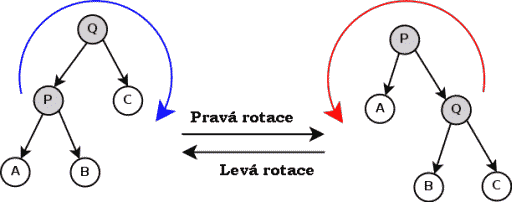
\includegraphics[width=12cm]{informatika/algoritmy_a_ds/obrazky/tree_rotation.png}

(Zdroj obrázku: Wikipedia)
\end{center}
\end{definiceN}


\begin{definiceN}{Červeno-černé stromy}
Červeno-černé stromy jsou binární vyhledávací stromy s garantovanou max. výškou $O(\log n)$, kde $n$ je počet uzlů, tj. operace na nich mohou mít asymptotickou časovou složitost $O(\log n)$. Pro jejich popis je nutné definovat \emph{interní uzly} - všechny uzly stromu a \emph{externí uzly} - na (interních) listech (a uzlech s jedním potomkem) uměle přidané NULLové ukazatele (de facto \uv{listy} červeno-černého stromu). Externí uzly slouží jenom jako abstrakce pro popis stromů, při implementaci se s nimi neoperuje. Červeno-černý strom má tyto čtyři povinné vlastnosti:
\begin{penumerate}
    \item Každý uzel (externí i interní) má definovanou barvu, a to černou nebo červenou.
    \item Každý externí uzel je černý.
    \item Každý červený vrchol musí mít oba syny černé.
    \item Každá cesta od libovolného vrcholu k listům v jeho podstromě musí obsahovat stejný počet černých uzlů.
\end{penumerate}

Pro červeno-černé stromy se definuje \emph{výška uzlu} $x$ ($\b{h}(x)$) jako počet uzlů na nedelší možné cestě k listu v jeho podstromě. \emph{Černá výška uzlu} ($\b{bh}(x)$) je počet černých uzlů na takové cestě.
\end{definiceN}

\begin{vetaN}{Vlastnosti červeno-černých stromů}
Podstrom libovolného uzlu $x$ obsahuje alespoň $2^{\b{bh}(x)}-1$ interních uzlů. Díky tomu má červeno-černý strom výšku vždy nejvýše $2\log(n+1)$ (kde $n$ je počet uzlů). (Důkaz prvního tvrzení indukcí podle $\b{h}(x)$, druhého z prvního a třetí vlastnosti červeno-černých stromů)
    \end{vetaN}

\begin{dusledek}
Operace hledání (minima, maxima, následníka, \dots), které jsou stejné jako u obecných binárních vyhledávacích stromů, mají garantovanou časovou složitost $O(\log n)$.
\end{dusledek}

\begin{algoritmusN}{Vkládání a odebírání uzlů v červeno černých stromech}
Obě operace mají podle garantované max. výšky garantovanou čas. složitost $O(\log n)$ pro $n$ počet uzlů. Protože bez porušení vlastností červeno-černých stromů lze kořen vždy přebarvit načerno, můžeme pro ně předpokládat, že \emph{kořen stromu} je \emph{vždy černý}.

\emph{Vkládání} vypadá následovně:
\begin{pitemize}
    \item Nalezení místa pro vložení a přidání nového prvku jako v obecných bin. vyhl. stromech, nový prvek se přebarví načerveno.
    \item Pokud je jeho otec černý, můžeme skončit -- vlastnosti stromů jsou splněné. Pokud je červený, musíme strom upravovat (tady předpokládám, že otec přidávaného uzlu je levým synem, opačný připad je symetrický):
    \item Je-li i strýc červený, přebarvit otce a strýce načerno a přenést chybu o patro výš (je-li děd černý, končím, jinak můžu pokračovat až do kořene, který už lze přebarvovat beztrestně).
    \item Je-li strýc černý a přidaný uzel je levým synem, udělat pravou rotaci na dědovi a přebarvit uzly tak, aby odpovídaly vlastnostem stromů.
    \item Je-li strýc černý a přidaný uzel je pravým synem, udělat levou rotaci na otci a převést tak na předchozí případ.
\end{pitemize}

\emph{Odebírání} se provádí takto:
\begin{pitemize}
    \item Odstraním uzel stejně jako v předchozím případě. Opravdu odstraněný uzel (z přepojování) má max. jednoho syna. Pokud odstraňovaný uzel byl červený, neporuším vlastnosti stromů, stejně tak pokud jeho syn byl červený -- to řeším jeho přebarvením načerno.
    \item V opačném případě (tj. syn odebíraného -- $x$ -- je černý) musím udělat násl. úpravy (přep. že $x$ je levým synem svého nového otce, v op. případě postupuji symetricky):
    \item $x$ prohlásím za \uv{dvojitě černý} a této vlastnosti se pokouším zbavit.
    \item Pokud je bratr $x$ (buď $w$) červený, pak má 2 černé syny -- provedu levou rotaci na rodiči $x$, prohodím barvy rodiče $x$ a uzlu $w$ a převedu tak situaci na jeden z násl. případů:
    \item Je-li $w$ černý a má-li 2 černé syny, prohlásím $x$ za černý a přebarvím $w$ načerveno, rodiče přebarvím buď na černo (a končím) nebo na \uv{dvojitě černou} a propaguji chybu (mohu dojít až do kořene, který lze přebarovat beztrestně).
    \item Je-li $w$ černý, jeho levý syn červený a pravý černý, vyměním barvy $w$ s jeho levým synem a na $w$ použiji pravou rotaci, čímž dostanu poslední případ:
    \item Je-li $w$ černý a jeho pravý syn červený, přebarvím pravého syna načerno, odstraním dvojitě černou z $x$, provedu levou rotaci na $w$ a pokud měl původně $w$ (a $x$) červeného otce, přebarvím $w$ načerveno a tohoto (teď už levého syna $w$) přebarvím načerno.
\end{pitemize}
\end{algoritmusN}


\begin{definiceN}{AVL stromy (Adelson-Velsky \& Landis)}
\emph{AVL stromy} jsou, podobně jako červeno-černé stromy, bin. vyhledávací stromy, které zaručují max. logaritmický nárůst výšky vzhledem k počtu prvků. Pro každý uzel $x$ se v AVL stromu definuje \emph{faktor vyvážení} jako rozdíl výšky jeho levého a pravého podstromu: $\b{bf}(x) = h(\texttt{x->levý}) - h(\texttt{x->pravý})$. Pro všechny uzly v AVL stromu platí, že $|\b{bf}(x)|\leq 1$.
\end{definiceN}

\begin{vetaN}{Zaručení výšky AVL stromů}
Výška AVL stromu s $n$ vrcholy je $O(\log n)$. (Důkaz: buď $T_n$ AVL strom výšky $n$ s minimálním počtem uzlů. Ten má podstromy $T_{n-1}$ a $T_{n-2}$ atd., tj. velikost minimálního AVL stromu roste jako Fibonacciho posloupnost, tedy $|T_n|\geq (\frac{1+\sqrt{5}}{2})^{n-1}$. Důkaz tohoto indukcí.)
\end{vetaN}

\begin{algoritmusN}{Operace na AVL stromech}
Vyhledávací operace se provádí stejně jako na obecných bin. vyhledávacích stromech, vkládání a odebírání prvků taky, ale pokud tyto operace poruší zákl. vlastnost AVL stromů ($|\b{bf}(x)=2|$), je nutné provést vyvažování -- pomocí rotací (které mohou být propagovány až ke kořeni). Při vkládání a odebírání je navíc nutné průběžně (nejhůře až ke kořeni) upravovat indikaci faktoru vyvážení jednotlivých uzlů.
\end{algoritmusN}

\subsubsection*{Halda}

\begin{definice}
\emph{Halda(heap)} je dynamická množina se stromovou strukturou (binární halda je binární strom), pro kterou platí tzv. \uv{vlastnost haldy}: $$\text{ Je-li }x\text{ potomek }y\text{, pak }x\texttt{->klíč}\geq y\texttt{->klíč}$$ Haldy s touto nerovností jsou tzv. \emph{min-heap}y, pokud je nerovnost opačná, jde o \emph{max-heap}.
\end{definice}

\begin{obecne}{(Binární) haldy}
Binární haldy jsou nejčastějším typem haldy. Zajišťují nalezení minimálního prvku v konstantním čase a odebrání a přidání minima v čase $O(\log n)$. V každé hladině od první až do předposlední je max. možný počet uzlů, v poslední jsou uzly co nejvíce \uv{vlevo} -- tedy max. výška haldy s $n$ prvky je $(\log n) + 1$. Proto je pro binární haldy jednoduše proveditelná jejich datová reprezentace polem (bez pointerů), kde při indexování od 0 má uzel na indexu $k$:
\begin{pitemize}
    \item Levého a pravého syna na indexu $2k+1$, resp. $2k+2$ (pokud to není víc než celk. počet prvků, potom syny nemá).
    \item Rodiče na indexu $\lceil\frac{k}{2}\rceil-1$. 
\end{pitemize}

\emph{Přidání uzlu} do haldy znamená přidání prvku na konec haldy a dokud má jeho rodič větší klíč, jeho prohazování s rodičem (tedy posouvání o vrstvu výš). Při \emph{odebírání uzlu} z haldy tento nahradím posledním prvkem v haldě a potom dokud neplatí vlastnost haldy (nejméně jeden z potomků má menší klíč), prohazuji ho s potomkem s menším klíčem (a posouvám o vrstvu níž).

Vytvoření haldy je možné v čase $O(n)$, kde $n$ je počet prvků v haldě -- přidání 1 prvku do haldy trvá $O(h)$, kde $h$ je aktuální výška (a $h$ roste od $0$ až k $\lceil\log n\rceil$, počet prvků ve výšce $k$ je $\frac{n}{2^{k+1}}$, bereme-li výšku listů rovnou nule) - v součtu za všechny prvky jde o $O(n\cdot\sum_{h=0}^{\lceil\log n\rceil}\frac{h}{2^h})$.

Binární halda se používá např. k \emph{třídění haldou} (heapsortu), kdy se z dat, která je potřeba utřídit, nejdříve postaví halda, a potom se opakuje operace odebrání kořene (tj. minimálního prvku).
\end{obecne}

\begin{obecne}{Fibonacciho haldy}
Fibonacciho haldy mají nízkou časovou složitost běžných operací -- amortizovaně $O(1)$ pro vložení, hledání minima apod.; odebrání prvku a odebrání minima má složitost $O(\log n)$ pro $n$ prvků v haldě. Tvoří ji skupina stromů, vyhovujících \uv{vlastnosti haldy}. Každý uzel haldy s $n$ prvky má max. $\log n$ potomků a ve svém podstromě minimálně $F_{k+2}$ uzlů, kde $F_k$ je $k$-té Fibonacciho číslo. To je zajištěno pravidlem, že při odebírání prvků lze z nekořenového uzlu oddělit max. 1 syna, jinak je nutné oddělit i tento uzel a ten se pak stane kořenem dalšího stromu. Počet stromů se snižuje při odebírání minima, kdy jsou spojovány dohromady.

Fibonacciho haldy se používají pro efektivní implementaci složitějších operací, jako např. Jarníkova nebo Dijkstrova algoritmu.
\end{obecne}

\newcommand{\nadpis}[1]{\pagebreak[2]\ramcek{\subsubsection*{#1}}}

\subsection{Hašování}

\begin{definiceN}{slovníkový problém} Dáno univerzum $U$, máme reprezentovat
$S \subseteq U$ a navrhnout algoritmy pro operace
\begin{pitemize}
\item MEMBER(x) - zjistí zda $x \in S$ a pokud ano nalezne kde,
\item INSERT(x) - pokud $x \notin S$, vloží $x$ do struktury reprezentující $S$,
\item DELETE(x) - když $x \in S$, smaže $x$ ze struktury reprezentující $S$.
\end{pitemize}
\end{definiceN}

Například pomocí pole můžeme tyto operace implementovat rychle, ale nevýhodou
je prostorová náročnost. Pro velké množiny je to někdy dokonce nemožné.
\emph{Hašování} se snaží zachovat rychlost operací a odstranit prostorovou
náročnost.

Podívejme se nyní na \emph{základní ideu} hašování. Mějme univerzum $U$ a
množinu $S \subseteq U$ takovou, že $|S| << |U|$. Dále mějme funkci
$h:U\rightarrow\{0,1,\dots,m-1\}$. Množinu $S$ potom reprezentujeme tabulkou
(polem) o velikosti $m$ tak, že prvek $x \in S$ je uložen na řádku $h(x)$.

\begin{definiceN}{Hašovací funkce, kolize} Funkci
$h:U\rightarrow\{0,1,\dots,m-1\}$ potom nazýváme \textbf{hašovací funkcí}.
Situaci $h(s)=h(t)$, pro $s \neq t; s,t \in S$  nazveme \textbf{kolize}.
\end{definiceN}

Jelikož mohutnost univerza $U$ je větší než velikost hašovací tabulky, nelze se
kolizím úplně vyhnout. Existuje spousta různých metod, jak kolize řešit.
Podívejme se tedy na některé podrobněji.

\begin{definice}
Ještě si zavedeme některé značení. Velikost $S$ (hašované množiny) označme
\textbf{n}, velikost tabulky (pole) označme \textbf{m}, a faktor naplnění
\textbf{$\alpha=\frac{n}{m}$}.
\end{definice}

\subsubsection*{Hašování se separovanými řetězci}

Použijeme pole velikosti $m$, jehož $i$-tá položka bude spojový seznam $S_i$
takový, že $s\in S_i \Leftrightarrow h(s)=i$, pro $s\in S$. Čili každý řádek
pole obsahuje spojový seznam všech (kolidujících) prvků, které jsou hašovány na
tento řádek. Seznamy nemusí být uspořádané, vznikají tak, jak jsou vkládány
jednotlivé prvky do struktury.

\begin{algoritmusN}{Hašování se separovanými řetězci}
\begin{pitemize}
\item \textbf{MEMBER} -- Spočteme hodnotu hašovací funkce $h(x)$, prohledáme
řetězec začínající na pozici $h(x)$ a zjistíme zda se prvek nachází, či
nenachází ve struktuře. Pokud se prvek v databázi nachází, tak musí nutně ležet
v tomto řetězci.
\item \textbf{INSERT} -- Zjistíme zda $x$ je v řetězci $h(x)$, pokud ne, přidáme
ho nakonec, v opačném případě neděláme nic.
\item \textbf{DELETE} -- Vyhledá $x$ v řetězci $h(x)$ a smaže ho. Pokud se tam
$x$ nenachází, neudělá nic.
\end{pitemize}
\end{algoritmusN}

\paragraph{Očekávaný počet testů} v neúspěšném případě je přibližně
$e^{-\alpha} + \alpha$ a při úspěšném vyhledávání přibližně
$1+\frac{\alpha}{2}$.

\subsubsection*{Hašování s uspořádanými řetězci}

Jak již je zřejmé z názvu je tato metoda téměř stejná jako předchozí. Jediný
rozdíl je, že jednotlivé seznamy jsou uspořádány vzestupně dle velikosti
prvků.

\begin{algoritmusN}{Hašování s uspořádanými řetězci}
Rozdíly jsou pouze pro operaci \textbf{MEMBER}, kde skončíme prohledávání, když
dojdeme na konec, nebo když nalezneme prvek, který je větší než hledaný a
operaci \textbf{INSERT}, které vkládá prvek na místo kde jsme ukončili
vyhledávání (před prvek, který ho ukončil).
\end{algoritmusN}

\paragraph{Očekávaný počet testů} v neúspěšném případě je přibližně roven
$e^{-\alpha}+1+\frac{\alpha}{2}-\frac{1}{\alpha}(1-e^{-\alpha})$ a v úspěšném
případě je přibližně $1+\frac{\alpha}{2}$.

Nevýhodou předchozích dvou metod je nerovnoměrné využití paměti. Zatímco
některé seznamy mohou být dlouhé, v některých není prvek žádný. Řešením je najít
způsob, jak kolidující prvky ukládat na jiné (prázdné) řádky tabulky. Potom je
ale nutné každý prvek tabulky rozšířit a položky pro práci s tabulkou. 

Čím použijeme sofistikovanější metodu ukládání dat do tabulky, tím více budeme
potřebovat položek pro práci s tabulkou a tedy vzroste paměťová náročnost. Naším
cílem je tedy najít rozumný kompromis mezi sofistikovaností (rychlostí)
strategie a její paměťovou náročností. Podívejme se na další algoritmy,
které se o to pokoušejí.

\subsubsection*{Hašování s přemísťováním}

Seznamy jsou tentokrát ukládány do tabulky a implementovány jako dvousměrné.
Potřebujeme tedy dvě položky pro práci s tabulkou: \emph{next} -- číslo řádku
obsahující další prvek seznamu a \emph{previous} -- číslo řádku obsahující
předchozí prvek seznamu. Když dojde ke kolizi, tj. chceme vložit prvek a jeho
místo je obsazené prvkem z jiného řetězce, pak tento prvek z jiného řetězce
přemístíme na jiný prázdný řádek v tabulce (proto hašování s přemísťováním).

\begin{algoritmusN}{Hašování s přemísťováním}
Algoritmus \textbf{MEMBER} funguje stejně jako u hašování se separovanými
řetězci, jen místo ukazatele na další prvek použije hodnotu \emph{next} z
tabulky. Při operaci \textbf{INSERT} vložíme prvek kam patří pokud je tam místo,
pokud již je místo obsazeno prvkem který tam patří, čili zde začíná seznam
kolidujících prvků (\emph{previous} = prázdné), pak postupujeme po položkách
\emph{next} až na konec seznamu, vložíme prvek na některý volný řádek
tabulky a vyplníme správně hodnoty \emph{next} a \emph{previous}. Pokud je místo
obsazeno prvkem z jiného seznamu (\emph{previous} $\neq$ prázdné), tak tento
prvek přemístíme na některý volný řádek, správně přepíšeme položky \emph{next} a
\emph{previous} v měněném seznamu a vkládaný prvek uložíme na jeho místo.
Operace \textbf{DELETE} je vcelku přímočará, jenom je třeba, pokud mažeme první
prvek seznamu na jeho místo přesunout ten druhý v pořadí (pokud existuje).
\end{algoritmusN}

\paragraph{Očekávaný počet testů} je v neúspěšném případě roven přibližně
$(1-\frac{1}{m})^n+\frac{n}{m}\approx e^{-\alpha}+\alpha$ a v úspěšném je stejný
jako pro hašování se separovanými řetězci a tedy $\frac{n-1}{2m}+1 \approx 1 +
\frac{1}{\alpha}$.

\subsubsection*{Hašování se dvěma ukazateli}

Hašování s přemísťováním má tu nevýhodu, že díky přemisťování prvků jsou operace
INSERT a DELETE časově náročné. Tato metoda tedy implementuje řetězce jako
jednosměrné seznamy, ale takové které nemusejí začínat na svém místě, tj.
řetězec $S_j$ obsahující prvky $s \in S$ takové, že $h(s)=j$, nemusí začínat na
$j$-tém řádku. Místo ukazatele na předchozí prvek tak do položek pro práci s
tabulkou přidáme ukazatel na místo, kde začíná řetězec příslušný danému řádku.
Položky pro práci s tabulkou tedy budou: \emph{next} -- číslo řádku tabulky kde
je další prvek seznamu, \emph{begin} -- číslo řádku tabulky obsahující první
prvek seznamu příslušného tomuto místu.

\begin{algoritmusN}{Hašování se dvěma ukazateli}
Položka \emph{begin} v $j$-tém řádku je vyplněna právě tehdy, když
reprezentovaná množina $S$ obsahuje prvek $s \in S$ takový, že $h(s)=j$.
Algoritmy jsou potom podobné těm u hašování s přemísťováním, ale přemísťování
prvků je nahrazeno odpovídajícími změnami v položce \emph{begin} daných řádků.
\end{algoritmusN}

Díky práci s položkami jsou operace INSERT a DELETE rychlejší než při hašování s
přemísťováním, ale začátek řetězce v jiném řádku tabulky přidá navíc jeden test,
což změní složitost operace MEMBER.

\paragraph{Očekávaný počet testů} v neúspěšném případě je přibližně
$1+\frac{\alpha^2}{2}+\alpha+e^{-\alpha}(2+\alpha)-2$ a při úspěšném vyhledávání
je roven $1+\frac{(n-1)(n-2)}{6m^2}+\frac{n-1}{2m} \approx 1 +
\frac{\alpha^2}{6}+\frac{\alpha}{2}$

\subsubsection*{Srůstající hašování}

Nyní se podíváme na několik verzí metody, která se nazývá srůstající hašování.
Budeme potřebovat jedinou položku pro práci s tabulkou a to ukazatel
jednosměrného spojového seznamu. Na rozdíl od předchozích metod zde nejsou
řetězce separované, v jednom řetězci mohou být prvky s různou hodnotou hašovací
funkce. Když máme přidat prvek $s$, tak ho zařadíme do řetězce, který se nachází
na $h(s)$-tém řádku tabulky. Řetězce tedy v této metodě \emph{srůstají}. Různé
verze této metody se liší tím, kam přidáváme nový prvek a podle práce s pamětí.
Dělí se na \emph{standardní srůstající hašování} bez pomocné paměti a na hašování
používající pomocnou paměť, kterému se říká jen \emph{srůstající hašování}.

Nejdříve se budeme věnovat metodám standardního srůstajícího hašování (bez
pomocné paměti):
\begin{pitemize}
\item \textbf{LISCH} -- late-insertion standard coalesced hashing -- vkládá se
za poslední prvek řetězce,
\item \textbf{EISCH} -- early-insertion standard coalesced hashing -- vkládá se
za první prvek řetězce.
\end{pitemize}

Přirozená efektivní operace DELETE pro standardní srůstající hašování není
známa. Na druhou stranu i primitivní algoritmy mají rozumnou očekávanou časovou
složitost.

Další otázka zní, proč používat metodu EISCH, když programy pro metodu LISCH
jsou jednodušší. Odpověď je na první pohled dost překvapující. Při úspěšném
vyhledávání je metoda EISCH rychlejší než metoda LISCH. Je to proto, že je o
něco pravděpodobnější, že se bude pracovat s novým prvkem. V neúspěšném případě
jsou samozřejmě obě metody stejné, neboť řetězce jsou u obou stejně dlouhé.

Metody srůstajícího hašování (s pomocnou pamětí) mají použitou paměť rozdělenou
na dvě části. Na tu přímo adresovatelnou hašovací funkcí a na pomocnou část.
Adresovací část má $m$ řádků, pokud hašovací funkce má hodnoty z oboru
$\{0,1,\dots,m-1\}$, v pomocné části jsou řádky ke kterým nemáme přístup přes
hašovací funkci. Když při přidávání nového prvku vznikne kolize, tak se nejprve
vybere volný řádek z pomocné části a teprve když je pomocné část zaplněna
použijí se k ukládání kolidujících prvků řádky z adresovatelné části tabulky.
Tato strategie oddaluje srůstání řetězců. Srůstající hašování se tedy, aspoň
dokud není zaplněna pomocná část tabulky, podobá hašování se separovanými
řetězci. Existují základní tři varianty:
\begin{pitemize}
\item \textbf{LICH} -- late-insertion coalesced hashing -- vkládá prvek na konec
řetězce,
\item \textbf{VICH} -- early-insertion coalesced hashing -- vkládá prvek na
řádek $h(x)$ pokud je prázdný a nebo hned za prvek na řádku $h(x)$,
\item \textbf{EICH} -- varied-insertion coalesced hashing -- vkládá se za
poslední prvek řetězce, který je ještě v pomocné části. Pokud v pomocné části
žádný není, vkládá se hned za prvek na pozici $h(x)$.
\end{pitemize}

Tyto metody nepodporují přirozené efektivní algoritmy pro operaci DELETE.

\subsubsection*{Hašování s lineárním přidáváním}

Následující metoda nepoužívá žádné položky pro práci s tabulkou to znamená, že
způsob nalezení dalšího řádku řetězce je zabudován přímo do metody. Metoda
funguje tak, že pokud chceme vložit prvek do tabulky a nastane kolize, najdeme
první následující volný řádek a tam prvek vložíme. Předpokládáme, že řádky jsou
číslovány modulo \emph{m}, čili vytvářejí cyklus délky \emph{m}.

Tato metoda sice využívá minimální velikost paměti, ale v tabulce vznikají
shluky obsazených řádků a proto je při velkém zaplnění pomalá. Navíc metoda
nepodporuje efektivní operaci DELETE.

\subsubsection*{Shrnutí}

Zde uvedeme pořadí metod hašování podle očekávaného počtu testů.

\begin{obecne}{Neúspěšné vyhledávání:}
\begin{penumerate}
\item Hašování s uspořádanými separovanými řetězci,
\item Hašování se separovanými řetězci = Hašování s přemísťováním,
\item Hašování se dvěma ukazateli,
\item VICH = LICH
\item EICH,
\item LISCH = EISCH,
\item Hašování s lineárním přidáváním.
\end{penumerate}
\end{obecne}

\begin{obecne}{Úspěšné vyhledávání}
\begin{penumerate}
\item H. s uspořádanými řetězci = H. se separovanými řetězci = H. s přemísťováním,
\item Hašování se dvěma ukazateli,
\item VICH,
\item LICH,
\item EICH,
\item EISCH,
\item LISCH,
\item Hašování s lineárním přidáváním.
\end{penumerate}
\end{obecne}

\begin{poznamka} Metody se separovanými řetězci a srůstající hašování používají
více paměti. Metoda s přemísťováním vyžaduje více času -- na přemístění prvku.
Otázka která z metod je nejlepší není proto jednoznačně rozhodnutelná a je nutné
pečlivě zvážit všechny okolnosti nasazení metody a všechny naše požadavky na ní,
než se rozhodneme, kterou použijeme.
\end{poznamka}

\subsubsection*{Univerzální hašování}

Pro dobré fungování hašování potřebujeme mimo jiné, aby vstupní data byla
rovnoměrně rozdělena a toho někdy není možné dosáhnout. Odstranit tento
nedostatek se pokouší metoda \emph{univerzální hašování}. Základní idea této
metody je taková, že máme množinu \emph{H} hašovacích funkcí z univerza do
tabulky velikosti \emph{m} takových, že pro $S \subseteq U$, $|S| \leq m$ se
většina funkcí chová dobře v tom smyslu, že má malý počet kolizí. Hašovací
funkci potom zvolíme z množiny \emph{H} (takovou s rovnoměrným rozdělením).
Jelikož funkci volíme my, můžeme požadavek rovnoměrného rozdělení zajistit.

\subsubsection*{Perfektní hašování}

Jiná možnost jak vyřešit kolize, je najít takzvanou \emph{perfektní hašovací
funkci}, tj. takovou které nepřipouští kolize. Nevýhoda této metody je, že nelze
dost dobře implementovat operaci INSERT, proto se dá prakticky použít pouze tam,
kde předpokládáme hodně operací MEMBER a jen velmi málo operací INSERT. Kolize
se potom dají řešit třeba malou pomocnou tabulkou, kam se ukládají kolidující
data. 

Pro rozumné fungování metody je nutné, aby hašovací funkce byla rychle
spočitatelná a aby její zadání nevyžadovat mnoho paměti, nejvýhodnější je
analytické zadání. 

Naopak jedna z výhod je, že nalezení perfektní hašovací funkce, může trvat
dlouho, neboť ho provádíme pouze jednou na začátku algoritmu. 

\subsubsection*{Externí hašování}

Externí hašování řeší trochu jiný problém, než výše popsané metody. Chceme
uložit data na externí médium a protože přístup k externím médiím je o několik
řádů pomalejší, než práce v interní paměti, bude naším cílem minimalizovat počet
přístupů do ní. Externí paměť bývá rozdělena na stránky a ty většinou načítáme
do interní paměti celé. Tato operace je však velice pomalá. Problémem externího
hašování je tedy nalézt datovou strukturu pro uložení dat na vnější paměti a
algoritmy pro operace INSERT, DELETE a MEMBER, tak abychom použili co nejmenší
počet komunikací mezi vnější a vnitřní pamětí.

Metod externího hašování je opět mnoho. Některé používají pomocnou datovou
strukturu v interní paměti, kterou často nazýváme adresář. Pokud metody nemají
žádnou takovou pomocnou strukturu neobejdou se obvykle bez oblasti přetečení.
Některé známější metody vnějšího hašování jsou například: \uv{Litwinovo lineární
hašování}, \uv{Faginovo rozšiřitelné hašování}, \uv{Cormackovo perfektní
hašování} nebo \uv{Perfektní hašování Larsona a Kajli}. 
% to neni preklep, hasovani je opravdu od pana KAJLI z nakyho duvodu se to uci
% blbe. viz http://portal.acm.org/citation.cfm?id=358193&coll=portal&dl=ACM
% ajs

\subsection{Sekvenční třídění, porovnávací algoritmy, přihrádkové třídění, třídící sítě}

TODO: trochu víc formalismu by tu neškodilo, taky je potřeba sjednotit óčkovou notaci (zřejmě prosté nahrazení symbolu $O$ symbolem $\Theta$ by stačilo, ale chce to ověřit).

\subsubsection*{Sekvenční třídění a porovnávací algoritmy}

Pojmy \uv{sekvenční třídění} a \uv{porovnávací algoritmy} mohou znamenat vlastně cokoliv, takže uvedu pár nejběžnějších třídících algoritmů a budu doufat, že to bude ke zkoušce stačit \texttt{:-(}. Zdrojem mi budiž Wikipedie a kniha Algoritmy a programovací techniky Doc. P. Töpfera.

\bigskip

\begin{algoritmusN}{Selection sort, třídění výběrem}
Selection sort je jeden z nejjednodušších třídích algoritmů. Jde o vnitřní třídění -- tedy celá posloupnost prvků by měla být v paměti. Má časovou složitost $\Theta(n^2)$ a obecně bývá pomalejší než insertion sort. Pracuje následovně:

Udržuje si množinu setříděných prvků na začátku posloupnosti (pole), která je na začátku prázdná a na konci představuje celé pole. Zbytek pole za setříděnou množinou je neuspořádaný. V jednom kroku vždy vybere jeden prvek a vloží ho do utříděné části (kterou tím zvětší o 1 a zároveň zmenší nesetříděnou). Jeden krok algoritmu (kterých je $n$ pro $n$ prvků v každém případě) vypadá takto: 
\begin{penumerate}
    \item Najdi nejmenší prvek z nesetříděného úseku.
    \item Vlož ho přesně za konec setříděného úseku (a prvek co tam byl původně si s ním vymění místo)
\end{penumerate}

Heapsort, který popíšu později, může být považovaný za variantu selection sortu, protože také vybírá minimum a začleňuje do setříděné části.
\end{algoritmusN}

\begin{algoritmusN}{Insertion sort, třídění vkládáním}
Insertion sort je také relativně jednoduchý a na velké datové soubory neefektivní, ale jednoduchý na implementaci a rychlejší než nejprimitivnější algoritmy bubble sort a selection sort. Navíc je efektivní pro data, která jsou už částečně předtříděná -- v nejhorším případě sice běží v čase $O(n^2)$, ale v nejlepším případě (úplné setřídění dat) je lineární -- obecně běží v čase $O(n+d)$, kde $d$ je počet inverzí ve tříděné posloupnosti. Navíc je stabilní (zachovává pořadí prvků se stejným klíčem) a \uv{in-place}, tedy nepotřebuje žádné pomocné datové struktury. Proti selection sortu ale většinou potřebuje více přepisování (a to může u velkých datových struktur vadit).

V jednom kroku vždy vezme nějaký prvek (berou se po řadě od začátku pole), zapamatuje si jeho hodnotu, a dokud před ním jsou prvky s větším klíčem, posouvá je na pozici o 1 větší (čímž vždy přepíše následující, takže původní prvek se ztratí) a pokud narazí na prvek s menším klíčem, do za něj napíše onen zapamatovaný prvek (a místo tam je, protože celou cestu k němu posouval prvky). Algoritmus vypadá takto:
\begin{verbatim}
insert sort( array a ){
  for( i = 1; i < a.length - 1; ++i ){
    value = a[i];
    j = i-1;
    while( j >= 0 && a[j] > value ){ 
      a[j + 1] = a[j];
      j = j-1;
    }
    a[j+1] = value;
  }
}
\end{verbatim}

Jednou z variant insertion sortu je \emph{Shell sort}, který porovnává prvky ne vedle sebe, ale vzdálené o nějaký počet polí, který se postupně zmenšuje. Může dosahovat složitost $O(n^{3/2})$ až $O(n^{4/3})$. S jistými úpravami se u něj dá dosáhnout až $O(n\log^2 n)$. Jiné vylepšení je \emph{library sort}, který si při vkládání nechává mezery pro další prvky (podobně jako v knihovně nejsou poličky úplně plné) -- ten může s velkou pravděpodobností běžet v čase $O(n\log n)$, ale zase potřebuje větší paměťový prostor.
\end{algoritmusN}

\begin{algoritmusN}{Bubble sort, bublinkové třídění}
Bubble sort je velmi jednoduchý třídící algoritmus (asi nejjednodušší na implementaci), s časovou složitostí $O(n^2)$. V nejlepším případě (pro úplně setříděná data) mu ale stačí jen jeden průchod, takže $O(n)$. Většinou ale bývá pomalejší i než insertion sort, takže se na velké množiny dat nehodí.

Algoritmus prochází v jednom kroku celé pole a hledá pozice, kde se prvek s menším klíčem nachází bezprostředně za prvkem s větším klíčem. Takovéto dva prvky pak vymění. Kroky opakuje, dokud neprojde celé pole bez jediného prohození prvků (nebo v \uv{tupější} variantě $n$-krát pro $n$ prvků, protože pak je zaručeno, že posloupnost bude pro libovolné pořadí prvků setříděná -- ta má ale pak složitost $O(n^2)$ v každém případě!).

Vylepšení algoritmu lze dosáhnout jednoduchou úvahou: největší prvek je už při prvním průchodu polem odsunutý až na konec. To se samozřejmě opakuje pro každý průchod (ve druhém je předposlední na druhém místě od konce atp.), takže lze průchody postupně zkracovat a konec pole už netestovat -- dosáhneme tím v průměru dvojnásobné rychlosti.

Variantou bubble sortu je \emph{shake sort} neboli \emph{cocktail sort}, který střídavě prochází posloupnost prvků nejdřív od začátku a pak od konce (a přitom provádí to samé jako bubble sort). Tím může v některých případech o trochu třídění zrychlit -- příkladem budiž posloupnost prvků $(2,3,4,5,1)$, která potřebuje jen 1 průchod cocktail-sortem tam a jeden zpět, ale pro bubble-sort by potřebovala 4.

Dalším vylepšením bubble sortu je \emph{Comb sort}, který o něco zvyšuje rychlost. Je založen na stejné myšlence jako shell sort -- tedy nejsou porovnávány prvky bezprostředně za sebou, ale prvky posunuté o nějaký ofset -- ten je na začátku roven délce posloupnosti, a postupně se dělí \uv{zkracovacím faktorem} (běžná hodnota $1.3$) až dosáhne jedné. Složitost se pohybuje mezi $O(n^2)$ v nejhorším případě a $O(n\log n)$ v nejlepším. V průměrném případě jde stále o $O(n^2)$, ale s menší konstantou než u bubble-sortu (TODO: tohle je potřeba set-sakra ověřit ... opsané z německé wiki a \uv{talk:Comb sort} na anglické, takže fakt \uv{důvěryhodné}).
\end{algoritmusN}

\begin{algoritmusN}{Heap sort, třídění haldou}
Heapsort je také třídící algoritmus založený na porovnávání a myšlenkově vychází ze selection sortu, ke kterému přidává práci s haldou. Většinou bývá pro typická vstupní data pomalejší než quicksort, ale zaručuje časovou složitost $O(n\log n)$ i v nejhorším případě. Jde o \uv{in-place} algoritmus (halda se může nacházet přímo v nesetříděné části pole), ale není \uv{stabilní}.

Algoritmus sám, máme-li vyřešené operace na haldě, je velice jednoduchý -- nejdříve pro každý prvek opakuje jeho vložení do haldy (takže postupně vytvoří $n$-prvkovou haldu, která se s každým krokem zvětšuje o 1), pro implementaci haldy na začátku pole je vhodný \uv{max-heap}, a potom opakuje odebrání maxima a jeho přesun na volné místo hned za konci zmenšivší se haldy -- takže od konce pole postupně roste směrem k začátku setříděná posloupnost.

Upravený heapsort s použitím ternární haldy dosahuje o multiplikativní konstantu lepší výsledky, existuje i (prý :-)) složitá varianta \emph{smoothsort}, která se blíží časové složitosti $O(n)$, pokud jsou data částečně předtříděná -- heapsort totiž pracuje pro libovolnou posloupnost v čase $O(n\log n)$.
\end{algoritmusN}

\begin{algoritmusN}{Merge sort, třídění sléváním}
Dalším třídícím algoritmem založeným na porovnávání prvků je mergesort. Je stabilní, takže zachovává pořadí dat se stejným klíčem. Jde o příklad algoritmu typu \uv{rozděl a panuj}, stejně jako u níže popsaného quicksortu. Byl vynalezen Johnem Von Neumannem. Je založen na rozdělení posloupnosti na dvě zhruba stejné poloviny, rekurzivním setřídění a potom \uv{slévání} dvou již setříděných posloupností. Jeho časová složitost je $O(n\log n)$ i v nejhorším případě, provádí většinou méně porovnání než quicksort, má větší nároky na paměť v případě rekurzivního volání (existuje ale i nerekurzivní verze), ale většinou nepracuje na místě a potřebuje alokovat paměť pro výstup setříděných posloupností (i toto se dá odstranit, ale je to zbytečně složité a přílišné zrychlení oproti použití jiného algoritmu nepřinese). Jeho přístup ho ale činí ideálním k použití na médiích se sekvenčním přístupem k datům (např. pásky). Jde tedy použít i ke třídění na vnější paměti -- detaily viz sekce o databázích.

Postup práce je následující:
\begin{penumerate}
    \item Rozděl nesetříděnou posloupnost na dvě (zhruba) poloviční části    
    \item Pokud mají více než jeden prvek, setřiď je rekurzivním zavoláním mergesortu (tj. pro každou z nich pokračuj od kroku 1 do konce algoritmu), jinak pokračuj následujícím krokem.
    \item Slij dvě setříděné posloupnosti do jedné -- vyber z obou posloupností první prvek, a pak opakovaně prvky porovnávej, zapisuj do setříděné posloupnosti menší z nich a doplňuj dvojici z té poloviční posloupnosti, odkud pocházel zapsaný prvek.
\end{penumerate}
\end{algoritmusN}

\begin{algoritmusN}{Quicksort}
Quicksort je jedním z nejrychlejších algoritmů pro třídění na vnitřní paměti, přestože v nejhorším případě může jeho časová složitost dosáhnout až $\Theta(n^2)$. Pro ideální i průměrná data dosahuje $\Theta(n\log n)$. Je také založen na principu \uv{rozděl a panuj}, i když poněkud jiným způsobem než předchozí zmiňovaný, od něhož se liší i tím, že není stabilní.

Algoritmus nejdřív vybere nějaký prvek, tzv. \emph{pivot}, a prvky s klíčem větší než pivot přesune do jiné části pole než ty s klíčem menším. Pak rekurzivně třídí obě části pole -- když se dostane k polím délky 1, problém je vyřešen. Postup vypadá takto:
\begin{penumerate}
    \item Vyber pivot (jeden prvek ze seznamu). Tady jde o největší magii, protože k dosažení nejlepší rychlosti by se měl pokaždé vybírat medián. Nejjednodušší je vybrat první, ale tento výběr ovlivňuje výslednou rychlost práce, takže se vyplatí např vzít tři prvky, porovnat je a vzít si z nich ten prostřední.
    \item Postupuj od začátku pole a hledej první prvek větší nebo rovný než pivot. Až ho najdeš, postupuj od konce a najdi první prvek menší než pivot. 
    \item Prvky prohoď a opakuj krok 2 a 3, dokud se hledání od začátku a od konce nepotká na nějaké pozici -- tu pojmenujeme třeba $k$.
    \item Rekurzivním voláním setřiď prvky $(0,\dots,k)$ a $(k+1,\dots,n-1)$ (má-li tříděné pole délku $n$) -- to znamená pro obě části pole pokračuj od kroku 1. Pokud je $k=0$ nebo $k=n-2$, není třeba už rekurzivního volání, protože posloupnosti délky 1 jsou setříděné.
\end{penumerate}

Pro algoritmus existuje i nerekurzivní verze (stačí rekurzi nahradit zásobníkem úseků čekajících na zpracování). Je vidět, že na volbě pivotu závisí všechno -- pokud pokaždé jako pivot volím 1. nebo $n-1$. hodnotu v poli v pořadí podle velikosti, dělím pak vždy na části o délce 1 a $n-1$, takže tento rekurzivní krok provedu až $n$-krát a dostanu se k času $\Theta(n^2)$. Samozřejmě, díky existenci algoritmu pro nalezení mediánu v čase $\Theta(n)$ je možné i tady dosáhnout zaručené složitosti $\Theta(n\log n)$, ale v praxi je to kvůli vysoké multiplikativní konstantě nepoužitelné -- k výběru pivotu se většinou s úspěchem užívá nějaká jednoduchá heuristika, jak je nastíněno v popisu algoritmu samotného.

Heapsort bývá pomalejší než quicksort, ale zaručuje nízkou časovou složitost i pro nejhorší případ a navíc potřebuje méně paměti -- nároky quicksortu navíc (kromě tříděné posloupnosti) jsou $O(\log n)$ minimálně, kvůli nutnosti použití rekurzivního volání nebo zásobníku. Oproti mergesortu ho nelze použít na data se sekvenčním přístupem, tyto nevýhody ale vyvažuje relativní jednoduchostí implementace a rychlostí v průměrném případě.

Variantou quicksortu je \emph{introsort}, který ho kombinuje s heapsortem, pokud hloubka rekurze dosáhne nějakých nepřijatelných hodnot -- tak je zaručena časová složitost $\Theta(n\log n)$ i v nejhorším případě (samozřejmě je to ale v nejhorším případě pořád pomalejší než použití jen heapsortu). Jedna z variant tohoto algoritmu se dá použít k hledání $k$-tého nejmenšího prvku (tedy i mediánu), kdy dosahuje složitosti $O(n)$ průměrně až $O(n^2)$ nejhůře.
\end{algoritmusN}


\subsubsection*{Přihrádkové třídění}

\begin{algoritmusN}{Bucket sort, Radix sort, přihrádkové třídění}
Radix sort je zvláštní třídící algoritmus -- jeho složitost je totiž lineární. Dosahuje to tím, že neporovnává všechny tříděné prvky (složitost problému třídění pomocí porovnávání je $\Theta(n\log n)$, takže by to jinak nebylo možné), je ho ale možné použít jen pro třídění dat podle klíče z nějaké ne příliš velké množiny -- max. rozsah tříděných hodnot závisí na tom, jak velké pole si můžeme dovolit vymezit v paměti pro tento účel.

Nejjednodušší varianta (tzv. \emph{pigeonhole sort}, nebo-li \emph{counting sort}) opravdu počítá s klíči ze zadaného rozmezí $[l,h]$. Pro něj si připraví cílové pole velikosti $h-l+1$, tj. \uv{přihrádky}. Do nich pak přímo podle klíče přehazuje čtené prvky (jestliže přihrádky realizujeme jako seznamy, bude třídění dokonce stabilní). Nakonec projde přihrádky od začátku do konce a co v nich najde, to vypíše (a výstup bude setříděný). Variantou counting sortu je \emph{bucket sort}, kdy se do jedné přihrádky nedávají jen prvky se stejným klíčem, ale prvky s klíčem v nějakém malém rozmezí -- ty pak lze setřídit rychle, protože jich zřejmě nebude mnoho, a navíc se ušetří paměť.


Protože ale klíče velikosti max. tisíců hodnot jsou většinou trochu málo, v praxi se běžně používají složitější varianty -- ty zahrnují několik průchodů nahoře popsaného algoritmu, při nichž se třídí jenom podle části klíče. Ty se dělí na ty, které začínají od nejméně významné části klíče (\emph{least significant digit radix sort}) a ty, které jdou od nejvýznamnější části (\emph{most significant digit}). První z nich mají tu výhodu, že lze zachovat stabilitu třídění, druhá zase může třídit i podle klíčů různé délky a zastavovat se po nalezení unikátních prefixů, takže se hodí např. pro lexikografické třídění podle řetězcových klíčů.

Třídění typu least significant digit vypadá následovně:
\begin{penumerate}
    \item Vezmi nejméně významnou část klíče (určitý počet bitů).
    \item Rozděl podle této části klíče data do přihrádek, ale v nich zachovej jejich pořadí (to je nutné kvůli následnému průchodu, zároveň to dělá z tohoto algoritmu stabilní třídění).
    \item Opakuj toto pro další (významnější) část klíče.
\end{penumerate}

Most significant digit varianta (rekurzivní verze, je založená na bucket sortu) běhá takto:
\begin{penumerate}
    \item Vezmi nejvýznamnější část klíče (první písmeno, například).
    \item Rozděl prvky podle této části do přihrádek (takže v jedné se jich octne docela hodně)
    \item Rekurzivně setřiď každou z přihrádek (začni podle další části klíče), pokud je v ní více než jeden prvek (tohle zaručí zastavení za rozlišujícím prefixem).
    \item Slep přihrádky do jedné (setříděné) posloupnosti.
\end{penumerate}

Popisované algoritmy většinou potřebují $O(n+(h-l))$ času k třídění, je-li $h-l$ (zhruba) počet přihrádek -- to znamená, že sice jde o složitost lineární, ale lineární i v počtu přihrádek, což se nemusí vždy oproti konvenčnímu třídění vyplatit. Navíc jsou problémem vysoké nároky na paměť (nelze třídění provést \uv{na místě} v jediném poli). Pro malou množinu hodnot klíčů (nebo u most significant digit varianty krátké odlišující prefixy) jsou ale časově efektivnější.
\end{algoritmusN}



\subsubsection*{Třídící sítě}

Zdrojem této sekce jsou zápisky z přednášek Prof. L. Kučery Algoritmy a datové struktury II.
\bigskip

\begin{definiceN}{Bitonická posloupnost}
Řekneme, že posloupnost prvků je \emph{bitonická}, pokud po spojení do cyklu (tedy nultý prvek za $n$-tý) obsahuje dva monotónní úseky. Nebo-li obsahuje až na fázový posuv dva monotónní úseky.
\end{definiceN}

\begin{definiceN}{Komparátor}
\emph{Komparátor} je speciální typ hradla (představme si pod tím nedělitelnou elektronickou součástku, případně jen virtuální), která má dva výstupy a dva vstupy. Pokud na vstupy přivedeme dva prvky (klíče, čísla), z levého výstupu vydá menší z nich a z pravého výstupu větší (takže vlastně porovná dva prvky a na výstup je vyplivne ve správném pořadí). Pracuje v konstantním čase.
\end{definiceN}

\begin{definiceN}{Třídící síť}
Třídící síť je správně sestavená množina komparátorů dohromady spojená vstupy a výstupy tak, že při přivedení posloupnosti délky $n$ na vstup ji vydá setříděnou na výstupu. Komparátory v ní jsou rozčleněné do hladin, jejichž počet pak udává celkovou dobu výpočtu -- předpokládá se tam, že komparátory v jednotlivých vrstvách pracují paralelně, takže třídící sítě mohou dosahovat časové složitosti pouhých $O(\log n)$. Algoritmus s takovou časovou složitostí sice existuje, ale má velmi vysokou multiplikativní konstantu, takže se v praxi nepoužívá. Příkladem třídící sítě je i bitonické třídění.
\end{definiceN}

\begin{algoritmusN}{Bitonické třídění}
Bitonická třídící síť je založena na použití bitonických posloupností a rekurze. Obvod (pro třídění dat délky $n$) se dělí na dvě části:
\begin{pitemize}
    \item První část setřídí (rekurzivně) $1/2$ vstupu vzestupně, druhou polovinu sestupně a tím vytvoří bitonickou posloupnost. Obsahuje tedy dvě třídící sítě pro třídění posloupností délky $\frac{n}{2}$.
    \item Druhá část třídí jen bitonické posloupnosti -- první její vrstva rozdělí bitonickou posloupnost na vstupu na dvě bitonické posloupnosti (z větších a menších čísel). Další vrstvy už jsou opět implementovány rekurzivně -- tedy druhá vrstva dostane dvě posloupnosti a vyrobí z nich čtyři atd., až nakonec dojde k \uv{bitonickým posloupnostem} délky 1.
\end{pitemize}

K rozdělení jedné bitonické posloupnosti délky $k$ na dvě stačí jen $\frac{k}{2}$ komparátorů, které porovnávají vždy $i$-tý a $k+i$-tý prvek. Dojde sice k nějakému fázovému posuvu, ale to ničemu nevadí. Dobře je to vidět při znázornění na kružnici, doporučuji prohlédnout si postup v programu Algovision Prof. Kučery (\texttt{http://kam.mff.cuni.cz/\~{}ludek/AlgovisionPage.html}).

Je vidět, že počet vrstev potřebných k dělení bitonických posloupností délky $N$ je $log_2 N$ ($B(N)=\log N$). Pro celkový počet vrstev, a tedy dobu zpracování -- $T(n)$ nám vychází následující vzorec
$$T(N) = T(\frac{n}{2}) + B(N) = \log N + \log(N/2) + \dots + 1$$
z čehož díky vzorci pro součet aritmetické posloupnosti $1+2+\dots+k=\frac{k(k+1)}{2}$ vyjde
$$T(N) = O(\frac{1}{2} \log^2 N)$$
\end{algoritmusN}

\def\Real{ \mathbb{R} }

\subsection{Grafové algoritmy}

TODO: nejake vyuziti tech algoritmu (staci priklad plusminus ke kazdemu druhu ulohy)

\subsubsection*{Graf}

\begin{definice}
\emph{Graf} $G$ je dvojice $(V,E)$, kde $V$ je množina bodů (\emph{vrcholů}) a $E$ množina jejich dvojic (\emph{hran}). Je-li $E$ množinou neuspořadaných dvojic, jde o \emph{neorientovaný} graf. Jsou-li dvojice uspořádané, jedná se o \emph{orientovaný} graf. Velikost množiny $V$ se značí $n$, velikost $E$ je $m$ - $|V|=n$, $|E|=m$. 

Graf je možné strojově reprezentovat např. pomocí \emph{matice sousednosti} -- matice, kde je na souřadnicích $(u,v)$ hodnota $1$, pokud z $u$ do $v$ je hrana a $0$ jinak. Pro neorientované grafy je souměrná podle hlavní osy. Matice zabírá $\Theta(n^2)$ místa v paměti. Další možností jsou \emph{seznamy sousedů} -- dvě pole, jedno příslušné vrcholům, druhé hranám. V prvním jsou uložené indexy do druhého pole, určující kde začínají seznamy hran vedoucích z vrcholu (příslušejícímu k indexu v prvním poli). Paměťová náročnost je $\Theta(m+n)$.
\end{definice}

\subsubsection*{Prohledávání do hloubky a do šířky}

Algoritmy, které postupně projdou všechny vrcholy daného souvislého neorientovaného grafu.

\begin{algoritmusN}{Prohledávání do šířky/Breadth-First Search}
Prochází všechny vrcholy grafu postupně po vrstvách vzdáleností od iniciálního vrcholu. K implementaci se používá fronta (FIFO).

\begin{verbatim}
BFS( V - vrcholy, E - hrany, s - startovací vrchol ){
  obarvi vrcholy bíle, nastav jim nekonečnou vzdálenost od s a předchůdce NULL;
  dej do fronty vrchol s;

  while( neprázdná fronta ){
    vyber z fronty vrchol v;
    foreach( všechny bíle obarvené sousedy v = u ){
       obarvi u šedě a nastav mu vzdálenost d(v) + 1 a předchůdce v;
       dej vrchol u do fronty;
    }
    v přebarvi na černo a vyhoď z fronty.
  }
}
\end{verbatim}


Běží v čase $\Theta(m+n)$, protože každý vrchol testuje 2x pro každou hranu, do fronty ho dává 1x a obarvení mu mění 2x. Tento algoritmus je základem několika dalších, např. pro testování souvislosti grafu, hledání minimální kostry nebo nejkratší cesty.
\end{algoritmusN}

\begin{algoritmusN}{Prohledávání do hloubky/Depth-First Search}
Prochází postupně všechny vrcholy - do hloubky (pro každý vrchol nejdřív navštíví první jeho nenavštívený    sousední vrchol, pak první sousední tohoto vrcholu atp. až dojde k vrcholu bez nenavštívených sousedů, pak se vrací a prochází další ještě nenavštívené sousedy). Pro implementaci se používá buď zásobník, nebo rekurze. Zásobníková verze vypadá stejně jako prohledávání do šířky (místo fronty je zásobník).

Rekurzivní verze - při zavolání na startovní vrchol projde celý graf:
\begin{verbatim}
DFS(v - vrchol){

  označ v jako navštívený;
  foreach( všechny nenavštívené sousedy v = u )
     DFS( u );
}
\end{verbatim}

Časová složitost je $\Theta(m+n)$, stejně jako u prohledávání do šířky.
\end{algoritmusN}


\subsubsection*{Souvislost}

\begin{definice}
\emph{Cesta} v grafu $G=(V,E)$ z vrcholu $a$ do vrcholu $b$ je posloupnost $v_0,v_1,\dots,v_n$ taková, že $v_0=a$, $v_n=b$ a pro všechna $v_i$, $i\in\{1,\dots,n\}$ je $(v_{i-1},v_i)\in E$. Graf $G=(V,E)$ je \emph{souvislý}, pokud pro každé dva vrcholy $u,v\in V$ existuje v $G$ cesta z $u$ do $v$. Toto platí pro orientované i neorientované grafy.
\end{definice}

\begin{algoritmusN}{Testování souvislosti grafu/počítání komponent souvislosti}
Algoritmus využívá prohledávání do šířky (nebo do hloubky) - v 1 kroku vždy najde dosud nenavštívený vrchol, začne z něj procházet graf a takto projde(oddělí) jednu komponentu souvislosti. Pokud skončí po prvním kroku, graf je souvislý. Počet kroků, potřebných k navštívení všech vrcholů grafu, je zároveň počtem komponent souvislosti.

Časová složitost je $\Theta(m+n)$, protože o algoritmu platí to samé co o prohledávání do šířky -- žádný vrchol nebude přidán do fronty více než jednou a testován více než 2x pro každou hranu.
\end{algoritmusN}


\subsubsection*{Topologické třídění}

\begin{definice}
\emph{Topologické uspořádání} vrcholů orientovaného grafu $G=(V,\overrightarrow{E})$ je funkce $t:V\to \{1,\dots,n\}$ taková, že pro každou hranu $(i,j)\in E$ je $t(i)<t(j)$. Lze provést pouze pro acyklické orientované grafy.
\end{definice}

\begin{algoritmusN}{Primitivní algoritmus}
V každém kroku najde vrchol, z něhož nevedou žádné hrany. Přiřadí mu nejvyšší volné číslo (začíná od $n$) a odstraní ho ze seznamu vrcholů. Uspořádání takto vytvořené je topologické, složitost algoritmu je $\Theta(n(m+n))$.
\end{algoritmusN}

\begin{algoritmusN}{Rychlý algoritmus}
K topologickému uspořádání se dá použít modifikace prohledávání do hloubky. Není třeba ani graf předem testovat na přítomnost cyklů, algoritmus toto objeví. Pro každý navštívený vrchol si poznamená čas jeho opuštění, uspořádání podle klesajících časů opuštění je topologické.
\begin{verbatim}
topologické_třídění( v - vrchol ) {

  global t; // čas opuštění, iniciální hodnota 0

  označ v jako navštívený;
  foreach ( u in sousední vrcholy v ) {
    if ( u je navštívený, ale ne opuštěný ) {
      chyba - cyklus;
      return;
    }
    else if ( u není navštívený )
      topologické_třídění( u );
  }
  označ v jako opuštěný v čase t;
  t = t + 1;
}
\end{verbatim}
Časová složitost zůstává stejná jako u prohledávání do šířky, tedy $\Theta(m+n)$, protože všechny kroky prováděné v rámci navštívení 1 vrcholu vyžadují jen konstatní počet operací.
\end{algoritmusN}

\begin{poznamka}
Topologické třídění se používá např. k zjištění nejvhodnějšího pořadí provedení navzájem závislých činností.
\end{poznamka}

\subsubsection*{Hledání nejkratší cesty v grafu}

\begin{definice}
\emph{Ohodnocení hran - váhová funkce} je funkce, která každé (orientované) hraně přiřazuje její \uv{délku} nebo \uv{cenu} jejího projití. Definuje se jako $w:E\to\Real$. \emph{Délka} (orientované) \emph{cesty} $p=v_0,v_1\dots,v_n$ v ohodnoceném grafu (grafu s váhovou funkcí) je potom $w(p)=\sum_{i=1}^n w(v_{i-1},v_i)$.

\emph{Vzdálenost} dvou vrcholů $u,v$ (\emph{váha nejkr. cesty} z $u$ do $v$) je $\delta(u,v) = \min\{ w(p)| p$ je cesta z $u \mbox{ do } v \}$, pokud nějaká cesta z $u$ do $v$ existuje, jinak $\delta(u,v)=\infty$. \emph{Nejkratší cesta} $p$ z $u$ do $v$ je taková, pro kterou $w(p)=\delta(u,v)$.
\end{definice}

\begin{poznamka}
Pro hledání nejkratší cesty v obecném grafu bez ohodnocení hran (tj. délka cesty je počet hran na ní) stačí prohledávání do šířky.
\end{poznamka}

\begin{algoritmusN}{Algoritmus kritické cesty (pro DAG)}
Pro hledání nejkratší cesty do všech bodů z jednoho zdroje v orientovaném acyklickém grafu (DAG) používá topologické třídění, které je pro takovýto graf proveditelné; spolu se zpřesňováním horních odhadů vzdáleností vrcholů.

Mám daný startovací vrchol $s$. Definuji $d(s,v)$ jako horní odhad vzdálenosti $s$ a $v$, tj. vždy $d(s,v)\geq\delta(s,v)$ pro lib. vrchol $v$. Hodnoty $d(s,v)$ před započetím výpočtu inicializuji na $+\infty$.

V algoritmu se provádí operace \uv{Relax}, znamenající zpřesnění odhadu $d(s,v)$ za použití cesty vedoucí z $s$ do $v$, končící hranou $(u,v)$ -- pokud má taková cesta nižší váhu než byl předchozí odhad $d(s,v)$, položím $d(s,v)=d(s,u)+w(u,v)$. Tato operace zachovává invariant $d(s,v)\geq\delta(s,v)$.

\begin{verbatim}
Relax (u, v) { //u = source, v = destination
  if (v.distance > u.distance + uv.weight) {
    v.distance := u.distance + uv.weight
    v.predecessor := u
  }
}
\end{verbatim}

\begin{verbatim}
kritická cesta( V - vrcholy, E - hrany, s - startovací vrchol ){

  topologicky setřiď V;
  inicializace - nastav d(s,v) = nekonečno pro všechny vrcholy;
  foreach( vrchol v, v pořadí podle top. třídění ){
    proveď operaci Relax za použití cest
        vedoucích do v přes všechna možná u;
  }
}
\end{verbatim} 

Výsledek dává nejkratší cesty díky topologickému setřídění grafu -- pro nejkr. cestu $p$ z $s$ do $v$ platí $t(v_i)<t(v_{i+1})$ a pokud mám $d(s,u)=\delta(s,u)$ a provedu Relax na $v$ podle $(u,v)$, pak dostanu $d(s,v)=\delta(s,v)$, z čehož se korektnost dá dokázat indukcí podle počtu hran na cestě.

Složitost algoritmu je $\Theta(n+m)$, protože taková je složitost topologického třídění a zbytek algoritmu každou hranu i každý vrchol testuje právě 1x.
\end{algoritmusN}

\begin{algoritmusN}{Dijkstrův algoritmus}
Pracuje na libovolném orientovaném grafu s nezáporným ohodnocením hran.
\begin{verbatim}
Dijkstra( V - vrcholy, E - hrany, s - startovací vrchol ){

   inicializace - nastav d(s,v) = nekonečno pro všechny vrcholy;
   S = prázdný; // množina "vyřízených" vrcholů
   Q = V;       // množina "nevyřízených" vrcholů

   while( Q není prázdná ){
      vyber u, vrchol s nejmenším d z množiny Q;
      vlož vrchol u do S;
      foreach( v, z u do v vede hrana )
        proveď operaci Relax pro v přes u;
   }
}
\end{verbatim}
Časová složitost při implementaci množin $S$ a $Q$ pomocí haldy je: $\Theta(n\cdot\log n)$ pro inicializaci ($n$ vložení do haldy), $\Theta(n\cdot\log n)$ celkem pro vybírání prvků s nejmenším $d$, jedno provedení Relax při změně $d$ trvá $\Theta(\log n)$ (úprava haldy) a provede se max. $m$-krát; tedy celkem $\Theta((m+n)\cdot\log n$).
\end{algoritmusN}

\begin{algoritmusN}{Bellman-Ford}
Bellman-Fordův algoritmus lze použít nejobecněji, ale je nejpomalejší. Funguje na libovolném grafu (pokud najde cyklus, jehož celková váha je záporná, a tedy nejkratší cesty nemají smysl, vrací chybu).

\begin{verbatim}
Bellman-Ford( V - vrcholy, E - hrany, s - startovací vrchol ){

  inicializace - nastav d(s,v) = nekonečno pro všechny vrcholy;
  d(s,s) = 0;
  
  // n-1 iterací, každá projde všechny hrany
  for( i = 1; i < |V|; ++i ) {
    foreach( hrana (u,v) z E )
      proveď operaci Relax pro v přes u;
  }

  // hledání záporného cyklu
  foreach( hrana (u,v) z E ){
    if ( d(v) > d(u) + w(u,v) ){
      chyba - záporný cyklus;
      return;
    }
  }
}
\end{verbatim}

Složitost algoritmu je $\Theta(m\cdot n)$. Vždy najde nejkratší cestu, protože v grafu bez záporných cyklů může mít cesta max. $n-1$ vrcholů. Důkaz nalezení záporného cyklu sporem, se sumou vah všech hran na něm (položím $<$ 0).
\end{algoritmusN}

\begin{poznamkaN}{Nejkratší cesty pro všechny dvojice vrcholů}
Pro hledání nejkratších cest pro všechny dvojice vrcholů lze buď použít $n$-krát běh některého z předchozích algoritmů, nebo \emph{Algoritmus \uv{násobení matic}} či \emph{Floyd-Warshallův algoritmus}. Ty oba používají matice sousednosti $W_G$ a počítají matici vzdáleností $D_G$. 

První z nich postupuje indukcí podle počtu hran na nejkr. cestě, vyrábí matice $D_G(x)$ pro $x$ hran na nejkratší cestě. $D_G(1)$ je $W_G$, pro výpočet kroku $i$ vždy $D_G(i-1)$ \uv{vynásobí} $D_G(1)$ použitím zvláštního \uv{násobení}, kde násobení hodnot je nahrazeno sčítáním a sčítání výběrem minima. Složitost je s využitím asociativity takto definovaného \uv{násobení} $\Theta(n^3\log n)$.

Floyd-Warshallův algoritmus jde indukcí podle velikosti množiny vrcholů, povolených jako vnitřní vrcholy na cestách. Používá $d_{u,v}(k)$ jako min. váhu cesty z $u$ do $v$ s vnitř. vrcholy z množiny $\{1,\dots,k\}$. V iniciálním kroku je taky $D_G(1)=W(G)$. Pro $i$-tý krok je $d_{u,v}(i)=\min\{d_{u,v}(i-1),d_{u,i}(i-1)+d_{i,v}(i-1)\}$. Složitost je $\Theta(n^3)$, navíc jeden krok je velice rychlý -- celkově je algoritmus většinou rychlejší než Bellman-Fordův a pro záporné cykly se časem na diagonále objeví záp. číslo, proto je není třeba testovat předem.
\end{poznamkaN}

\subsubsection*{Minimální kostra grafu}

Úkolem v této úloze je najít kostru $T$ (acyklický souvislý podgraf) grafu $(V,E)$ s celkovou minimální vahou hran. Vždy platí $|T|=|V|-1$. Bez újmy na obecnosti lze předpokládat, že ohodnocení hran jsou nezáporná (lze ke všem přičíst konstantu a výsledek se nezmění).

\begin{algoritmusN}{Borůvkův / Kruskalův algoritmus}
\begin{verbatim}
Borůvka( V - vrcholy, E - hrany ){

  S = setříděné hrany podle jejich váhy;
  přiřaď vrcholům čísla komponent souvislosti;
  F = {};     // tj. (V,F) je "les", kde každý vrchol je 
               // jedna komponenta souvislosti
  
  while( S není prázdná ){
    vyber z S další hranu (x,y);
    if ( číslo komponenty x != číslo komponenty y ){
      F += (x,y);
      slij komponenty příslušné k x a y;
    }
  } 
  return ( (V,F) jako minimální kostru (v,E) );
}
\end{verbatim}

Celková složitost je $\Theta(m\log m)$ při použití spojových seznamů: Setřídění hran podle váhy $\Theta(m\log m)$, nalezení čísla komponenty konstantní čas, max. počet přečíslování komponent při slévání (přečíslovávám-li vždy menší ze slévaných komponent) pro 1 vrchol je $\Theta(\log n)$, tj. celkem $\Theta(n\log n)$.

Algoritmus je korektní - vždy nalezne kostru, protože přidá právě $|V|-1$ hran a nevytvoří nikdy cyklus. Minimalita kostry se dokáže sporem -- mám-li $F$ vrácenou algoritmem a $H$ nějakou min. kostru, tak pokud je $w(F)>w(H)$, najdu hranu $e\in F\setminus H$, vezmu kostru $H_1=H\cup e\setminus f$ (a $w(e)\leq w(f)$). Pokud mám $\forall e$ nalezené $f$ takové, že $w(e)=w(f)$, jsou $F$ i $H$ minimální, jinak $H$ taky nebylo minimální, protože $H_1$ je menší.
\end{algoritmusN}

\begin{algoritmusN}{Jarníkův / Primův algoritmus }
\begin{verbatim}
Jarník( V - vrcholy, E - hrany, r - startovní vrchol ){

  Q = V;  // množina používaných vrcholů, dosud nepřipojených
          // ke kostře
  F = {}; // vznikající kostra, v každém okamžiku 
          // je strom

  inicializace - nastav klíč(v) na nekonečno
      pro všechny vrcholy;
  klíč(r) = 0;
  soused(r) = NULL;

  while( Q je neprázdná ){
    vyber u, prvek s nejmenším klíčem z Q;
    F += ( soused(u),u );
    foreach( vrchol v, z u do v vede hrana ){
      if ( v je v Q a klíč(v) > w(u,v) ){
         klíč(v) = w(u,v);
         soused(v) = u;
      }
    }
  }
  return ( (V,F) jako min. kostru (V,E) );
}
\end{verbatim}

Složitost algoritmu je $\Theta(m\log n)$, pokud je $Q$ reprezentováno jako bin. halda - nejvýše $m$-krát upravuji klíč nějakého vrcholu, což má v haldě složitost $\Theta(\log n)$, výběr minima max. $n$-krát $\Theta(\log n)$ a inicializace jen $\Theta(n)$.

Vytvořený graf je kostra, protože nikdy nevzniká cyklus (připojuji právě vrcholy z $Q$, která je na konci prázdná). Důkaz minimality podle konstrukce -- najdu první hranu $e$ v min. kostře $H$, která není ve výsledku alg. $F$, pak najdu $f\in H$, t.ž.  $F\setminus e\cup f$ je kostra, z algoritmu je $w(f)\geq w(e)$. Vezmu $H_1=H\setminus f\cup e$, vím, že $w(H_1)\leq w(H)$ a tedy $H_1$ je min. kostra, iterací tohoto postupně dostanu, že $H_k=F$ je min. kostra.
\end{algoritmusN}


\subsubsection*{Toky v sítích}

\emph{není požadaváno v IP a ISPS}

\begin{definiceN}{Síť, tok}
\emph{Síť} je čtveřice $(G,z,s,c)$, kde $G$ je (orientovaný) graf, $z$ zdrojový a $s$ cílový vrchol (stok, spotřebič) a $c:E\to\Real^{+}$ funkce kapacity hran. \emph{Tok} sítí je taková funkce $t:E\to\Real^{+}$, že pro každou hranu $(u,v)$ je $0\leq t((u,v))\leq c((u,v))$ a navíc pro každý vrchol $v$ kromě $z$ a $s$ (\emph{uzel sítě}) platí $\sum_{e=(u,v)}t(e) = \sum_{e=(v,w)}t(e)$ (tj. \emph{přebytek toku} - rozdíl toho co do vrcholu vteče a co z něj odteče $\delta(t,v)$ je pro uzly sítě nulový). \emph{Velikost toku} se definuje jako $|t|=\delta(t,s)$.
\end{definiceN}

\begin{algoritmusN}{Ford-Fulkersonův algoritmus}
Algoritmus používá myšlenku zlepšitelné cesty - tj. pokud existuje v grafu neorientovaná cesta ze $z$ do $s$ taková, že pro hrany ve směru od zdroje je $t<c$ a pro hrany ve směru ke zdroji $t>0$, pak mohu tok zlepšit (o minimum rezerv). Algoritmus opakuje takovýto krok, dokud je možné ho provést. Neřeší výběr cesty, proto je dost pomalý a pokud nejsou hodnoty $t$ racionální čísla, může se i zacyklit.

Ve chvíli zastavení algoritmu získám max. tok, neboť množina $A=\{ v|$ ze $z$ do $v$ vede zlepšitelná cesta $\}$ je v tom okamžiku \emph{řez} (množina $A\subset V$ taková, že $z\in V$, $s\notin V$) a jeho \emph{velikost} ($\sum_{e\in E}c(e),e=(u,v),u\in A,v\notin A$) je stejná jako velikost získaného toku.
\end{algoritmusN}


\begin{algoritmusN}{Dinitzův algoritmus}
Řeší výběr zlepšitelné cesty -- vybírá vždy nejkratší cestu (což obecně popisuje \emph{Edmunds-Karpův algoritmus}). Dinitzova varianta používá \emph{síť rezerv}, což je graf $(V,R)$, kde hrana $e=(v,w)\in R$, pokud má tok hranou kladnou \emph{rezervu}, tj. $r = c(v,w)-t(v,w)+t(w,v) > 0$. Zlepšující cesta odpovídá normální orientované cestě v síti rezerv. Převod na pův. graf ze sítě rezerv je jednoduchý, mohu předpokládat, že jedním ze směrů mezi dvěma vrcholy neteče nic.

Průběh algoritmu: na začátku nastaví všem hranám rezervu $r(v,w)=c(v,w)$. Potom postupuje po \emph{fázích} - v 1 fázi:
\begin{pitemize}
\item Vyhodí ze sítě rezerv všechny hrany, které nejsou na nejkratší cestě $z\to s$ (2x prohledávání do šířky).
\item Vezme jednu z nejkr. cest v síti rezerv a zlepší podle ní tok.
\item Vyhodí vzniklé slepé cesty v síti rezerv (testuji jen hrany, co vyhazuji, a jejich konc. vrcholy)
\item Toto opakuje, dokud jsou v síti rezerv cesty $z\to s$ dané nejkratší délky.
\end{pitemize}
Další fází algoritmus pokračuje, dokud existuje vůbec nějaká cesta $z\to s$ v síti rezerv. Fází je tím pádem max. $n$ (max. délka cesty ze $z$ do  $s$), v 1 fázi se prochází max. $m$ cest (klesá počet použitelných hran), nalezení 1 cesty je $O(n)$ (jdu přímo) a vyhazování slepých cest max $O(m)$ celkem za fázi (každou hranu vyhodím jen jednou). Celková složitost je tedy $O(n^2 m)$.
\end{algoritmusN}


\begin{algoritmusN}{Goldbergův algoritmus (preflow-push, algoritmus vlny)}
Nehledá v grafu zlepšující cesty, v průběhu výpočtu v grafu není tok, ale vlna (ze zdroje teče vždy více nebo rovno než max. tok). \emph{Preflow} -- \uv{vlna} -- je funkce $t:E\to\Real^{+}$ taková, že $\forall e\in E: 0\leq t(e)\leq c(e)$, tedy přebytky toku ve vrcholech ($\delta$) jsou povolené. Ve chvíli, kdy žádný vrchol nemá přebytek toku ($\delta$), dostávám (maximální) tok. Pro každý vrchol $v$ si algoritmus pamatuje \uv{výšku} $h(v)$.  Také pracuje se sítí rezerv.
\begin{pitemize}
    \item \emph{Inicializace}: $h(z)=n$, $h(v,v\neq z)=0$, $t(e)=0\ \forall e$, $\delta(v)=0\ \forall v$.
    \item \emph{Úvodní preflow}: převede ze zdroje maximum možného ($t(e)=c(e)$ po směru) do sousedních vrcholů.
    \item \emph{Hlavní cyklus}: opakuje se, dokud existuje vnitřní vrchol $v$ s kladným $\delta$. pro vrchol $v$:
    \begin{pitemize}
        \item pokud existuje hrana $(v,w)$ nebo $(w,v)$, t.ž. $r(e) > 0$ (v daném směru) a $h(v)\geq h(w)$, potom se převede $\min(\delta(v),r(e))$ z $v$ do $w$.
	\item jinak se zvýší $h(v)$ o 1.
    \end{pitemize}
\end{pitemize}

Po celou dobu běhu algoritmu platí invariant $e=(v,w),r(e)>0\ \Rightarrow\ h(v)\leq 1+h(w)$. To zaručuje, že nalezený tok po zastavení je maximální (zdroj je ve výšce $n$, stok $0$, tedy každá cesta překonává někde rozdíl $-2$). Vrcholy nejde zvedat donekonečna, takže se algoritmus zastaví: pro každý vnitřní vrchol $v$ platí, že je-li $\delta(v)>0$, pak existuje v síti rezerv cesta $v\to z$. To zaručuje, že $h(v)\leq 2n-1$ - pokud mám vrchol $v$ tak, že $h(v)=2n-1$ a $\delta(v)>0$, potom existuje cesta $v\to z$ s kladnými rezervami a podle invariantu jde každá hrana na ní max. o 1 nahoru (tedy max. o $n-1$ celkem).

Složitost Goldbergova algoritmu je $O(n^2\cdot m)$.
\end{algoritmusN}

\subsection{Tranzitivní uzávěr}

\begin{definice}
  \textbf{Tranzitivní uzávěr} orientovaného grafu je orientovaný graf s
  původními vrcholy a platí, že existuje hrana z uzlu \emph{u} do uzlu \emph{v}
  právě tehdy, když v původním orientovaném grafu existuje libovolná orientovaná
  cesta z uzlu \emph{u} do uzlu \emph{v}.
\end{definice}

\begin{figure}[!ht]
  \begin{center}
    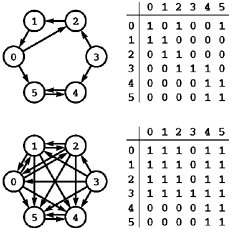
\includegraphics[scale=.7]{informatika/teoreticka_informatika/obrazky/tranzuzaver.png}
    \caption{Tranzitivní uzávěr grafu (zdroj: http://zorro.fme.vutbr.cz/graphs/foil36.html)}
  \end{center}
\end{figure}

\begin{poznamka}
  Platí, že matice dosažitelnosti v grafu $G$ = matice sousednosti tranzitivního
  uzávěru grafu $G$.
\end{poznamka}

\begin{obecne}{Algoritmus}
Z každého vrcholu vypustit DFS (Depth-first search~-- prohledávání do hloubky), do společné matice zaznamenávat dosažené vrcholy (řádek odpovídá vrcholu, sloupce vrcholům, které jsou z něho dosažitelné) -- složitost $O(n(n+m))$.
\end{obecne}

\begin{obecne}{Warshallův algoritmus}
Iterativní konstrukce matice dosažitelnosti, postupně počítá matice $W_k$, kde $w^{[k]}_{i, j} = 1$, pokud mezi vrcholy $i$ a $j$ existuje cesta, jejíž všechny vnitřní vrcholy jsou mezi vrcholy $1\dots k$.

Z matice $W_k$ lze spočítat matici $W^{[k+1]}: W^{[k+1]}_{i,j} = W^{[k]}_{i,j}  || (W^{[k]}_{i,k+1} \&\& W^{[k]}_{k+1,j})$ -- buď vede mezi vrcholy $i, j$ cesta, která nepoužije vrchol $k+1$, nebo taková, která ho použije -- v tom případě ale musí vést cesty mezi vrcholy $i,k+1$ a $k+1,j$, které používají pouze vrcholy $1\dots k$, jejich spojením je cesta mezi vrcholy $i,j$

Matice $W^1$ je matice incidence původního grafu.

Pseudokód (vstup: I -- matice incidence, $[0,1]^{n\times n}$):
\begin{verbatim}
Procedure Warshall(I)
W:= I;
for k:=1 to n
begin
  for i:=1 to n
  begin
    for j:=1 to n
\end{verbatim}
      $w_{i,j} = w_{i,j} || (w_{i,k} \&\& w_{k,j})$
\begin{verbatim}
  end
end 
return W;
\end{verbatim}

Složitost algoritmu je jasně $O(n^3)$ (potřebuje $2n^3$ bitových operací), což může být lepší pro grafy s hodně hranami (počet hran se blíží $n^2$), než složitost $n*DFS$ ( $n*(n + m) ≈ n * (n + n^2) = n^2 + n^3$ )

\end{obecne}

TODO: ještě něco?

\subsection{Algoritmy vyhledávání v textu}
Toto sú len veľmi stručné výťahy z wikipedie. Aktuálne sú tu len preto, aby si človek rýchlo vybavil, o čom tie algoritmy sú :-)

\subsubsection*{Rabin-Karp}
Umožňuje vyhľadávanie viacerých reťazcov v texte naraz - užitočné napr. na hľadanie plagiátov. Základnou myšlienkou je vyhľadávanie v texte pomocou hashov (rolling hashes - idea je \texttt{s[i+1..i+m] = s[i..i+m-1] - s[i] + s[i+m]})...

Algoritmus pre vyhľadávanie jedného reťazca:
\begin{verbatim}
 1 function RabinKarp(string s[1..n], string sub[1..m])
 2     hsub := hash(sub[1..m])
 3     hs := hash(s[1..m])
 4     for i from 1 to n-m+1
 5         if hs = hsub
 6             if s[i..i+m-1] = sub
 7                 return i
 8         hs := hash(s[i+1..i+m])
 9     return not found
\end{verbatim}

Najhoršia zložitosť je $\Omega(mn)$. Pri vyhľadávaní viacerých reťazcov len spočítame hashe všekých hľadaných stringov a pri nájdení niektorého z hashov príslušný reťazec porovnáme s textom... Ostatné algoritmy spotrebujú čas $O(n)$ na nájdenie 1 reťazca a teda $O(nk)$ na vyhľadanie $k$ reťazcov. Naproti tomu tento algoritmus má očakávanú zložitosť $O(n+k)$ - pretože vyhľadávanie v hashovacej tabuľke, či je hash podreťazca textu rovný hashu niektorého z hľadaného reťazcov, trvá $O(1)$.

\subsubsection*{Aho-Corasick}

Dokáže vyhľadávať viacero reťazcov naraz - používa na to trie-like štruktúru (konečný automat), ktorý obsahuje nasledujúce \uv{prvky}:
\begin{penumerate}
	\item konečná množina $Q$ - stavy
	\item konečná abeceda $A$
	\item transition funkcia $g$: $Q \times A \rightarrow Q + \{fail\}$
	\item failure funkcia $h$: $Q \rightarrow Q + \{fail\}$. $h(q)=q'$ práve vtedy keď spomedzi všetkých stavov Q dáva $q'$ najdlhší suffix z $path(q)$.
	\item konečná množina $F$ - koncové stavy
\end{penumerate}

Príklad \uv{hotového} automatu pre slová P=\{ab, ba, babb, bb\}:

\par\begin{center}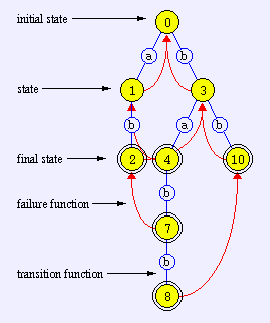
\includegraphics[width=8cm]{informatika/algoritmy_a_ds/obrazky/ahocorasick-automatron.png}\end{center}

Zložitosť vyhľadávania je lineárna vzhľadom k dĺžke textu a počtu nájdených \uv{slov} (pozn.: ten môže byť až kvadradický - slovník a, aa, aaa, aaaa; reťazec aaaa). Trie štruktúru je možné vyrobiť raz a potom používať počas vyhľadávania - uchovávame si najdlší match a používame suffix odkazy (aby sme udržali linearitu výpočtu).

Výstavba stromu se provede prostým zařazováním slov do trie-stromu podle prefixů. Na této struktuře je potom možné v lineárním čase (vzhledem k počtu znaků hledaných slov) předpočítat hodnoty failure funkce: automat vždy pustíme na sufix aktuálně zkoušeného slova, bez prvního znaku. Díky tomu, že průběžně ukládáme hodnoty nalezených slov, pro každé písmeno provede max. 2 kroky (postup vpřed a uložení hodnoty, kam bych spadnul).


\subsubsection*{Knuth-Morris-Pratt}

Obdoba Aho-Corasick, ale hľadá len jedno slovo. Samozrejme nie je potrebná dopredná funkcia (vždy iba nasledujúci znak), používa sa \uv{partial match} tabuľka (failure funkcia).

\begin{verbatim}
algorithm kmp_search:
    input:
        S (the text to be searched)
        W (the word sought)

    m = 0 (the beginning of the current match in S)
    i = 0 (the position of the current character in W)
    an array of integers, T (the table, computed elsewhere)

    while m + i is less than the length of S, do:
        if W[i] = S[m + i],
            i = i + 1
            if i equals the length of W,
                return m
        otherwise,
            m = m + i - T[i],
            if i is greater than 0,
                i = T[i]

    (if we reach here, we have searched all of S unsuccessfully)
    return the length of S
\end{verbatim}

Zložitosť algoritmu je je $O(k)$ (k je dĺžka S) - cyklus je vykonaný najviac $2k$ krát.

Algoritmus na výrobu tabuľky:
\begin{verbatim}
algorithm kmp_table:
    input:
        W (the word to be analyzed)
        T (the table to be filled)

    i = 2 (the current position we are computing in T)
    j = 0 (the zero-based index in W of the next
           character of the current candidate substring)

    (the first few values are fixed but different
          from what the algorithm might suggest)
    let T[0] = -1
    T[1] = 0

    while i is less than the length of W, do:
        (first case: the substring continues)
        if W[i - 1] = W[j],
            T[i] = j + 1
            i = i + 1
            j = j + 1

        (second case: it doesn't, but we can fall back)
        otherwise, if j > 0,
            j = T[j]

        (third case: we have run out of candidates. Note j = 0)
        otherwise,
            T[i] = 0
            i = i + 1
\end{verbatim}


Zložitosť tohoto algoritmu je $O(n)$ (n je dĺžka W) - cyklus skončí najviac po $2n$ iteráciách.

\subsection{Algebraické algoritmy}

\subsubsection*{Diskrétní Fourierova Transformace (DFT)}

Diskrétní Fourierova transformace se používá, chceme-li zachytit hodnotu (přepokládejme, že $2\pi$-periodické) funkce na intervalu $[-\pi,\pi]$ v nějakých $n$ bodech. To je dobré např. pro vzorkování elektrického nebo zvukového signálu a jiné operace. Pro nějakou funkci nám tak stačí znát vektor dimenze $n$ (a $n$ je počet vzorků na $2\pi$).

Je to založeno na Fourierových řadách -- dá se ukázat, že funkce $1$, $\cos kx$ a $\sin kx$ pro $k\geq 1$ tvoří ortogonální bázi prostoru spojitých funkcí na intervalu $[-\pi,\pi]$. Protože potřebujeme znát jenom konečný počet vzorků, stačí nám jen konečný podprostor s konečnou bází. Máme-li rozklad nějaké $2\pi$-periodické funkce do Fourierovy řady $f(x)= c + \sum_{k=1}^\infty a_k \sin k x + \sum_{k=1}^\infty b_k \cos k x$, dá se jednoduše ukázat, že pro hodnoty v bodech $-\pi,-\pi + \frac{\pi}{n}, -\pi + 2\frac{\pi}{n}, \dots, -\pi + (n-1)\frac{\pi}{n}$ stačí sumy do $\frac{n}{2}-1$ pro sinusové řady a $\frac{n}{2}$ pro kosinové -- vyšší koeficienty v takových bodech jsou nulové. Takže $n$ hodnot funkce $f$ na intervalu $[-\pi,\pi]$ lze reprezentovat vektorem $n$ čísel v bázi $1,\cos x,\dots,\cos \frac{n}{2}x,\sin x,\dots,\sin(\frac{n}{2}-1)x$. 

Jednodušeji to lze ukázat v komplexních číslech -- je známo, že 
$$e^{ix} = \cos x+ i\cdot\sin x$$
takže vektor hodnot funkce lze ekvivalentně reprezentovat v bázi $e^{i\cdot 2\pi\frac{k}{n}},\ k\in\{0,\dots,n\}$, neboť všechny vektory původní báze lze zapsat jako lineární kombinace vektorů nové báze. Definujeme hodnotu
$$\omega := e^{i\cdot 2\pi\frac{1}{n}} \textrm{ (a to je vlastně \uv{něco jako} }\sqrt[n]{1}\textrm{)}$$
vidíme, že $\omega^k$ je $n$-periodická funkce, takže nezáleží na hranicích sumace ($-\frac{n}{2}+1,\dots,\frac{n}{2}$ je ekvivalentní $0,\dots,n-1$). 
Potom se posloupnost $n$ komplexních čísel $\alpha_0, \dots, \alpha_{n-1}$ (např. hodnot naší funkce v bodech $-\pi + \frac{2\pi k}{n},\ k\in\{0,\dots,n-1\}$) transformuje na posloupnost $n$ komplexních čísel $A_0, \dots, A_{n-1}$ (do báze $\omega^i,\ i\in\{0,\dots,n-1\}$) použitím vzorečku:
$$A_j = \sum_{k=0}^{n-1} \alpha_k \omega^{kj}  \;\;\;\;\; j = 0, \dots, n-1$$
Tento převod označujeme jako \emph{diskrétní Fourierovu transformaci}.

\emph{Inverzní diskrétní Fourierova transformace} je opačný problém -- z $n$ Fourierových koeficientů $A_k$ chceme zpětně vypočítat hodnoty funkce $\alpha_k$ v bodech $-\pi + \frac{2\pi k}{n},\ k\in\{0,\dots,n-1$. Platí:

$$\alpha_j = \frac{1}{n}\sum_{k=0}^{n-1} A_k \omega^{-kj}  \;\;\;\;\; j = 0, \dots, n-1$$

\medskip
\begin{dukaz}
Definujeme matici $W: W_{p,q}=\omega^{pq}$, potom $A = W\alpha$ (vektorově), takže $a = W^{-1}A$. Definujeme $W': W'_{p,q}=\omega^{-pq}$ a dokážeme, že $W\cdot W'= n\cdot I_n$. Máme
$$(W\cdot W')_{p,q} = \sum_{s=0}^{n-1} W_{p,s}\cdot W'_{s,q} = \sum_{s=0}^{n-1} \omega^{(p-q)\cdot s}$$
a potom pro
\begin{pitemize}
    \item $p = q$ platí $\sum_{s=0}^{n-1}\omega^{(p-q)\cdot s} = \sum_{s=0}^{n-1}\omega^0 = \sum_{s=0}^{n-1} 1 = n$
    \item $p\neq q$ definujeme
    $$Q:= \omega^{p-q}$$
    a dostaneme geometrickou posloupnost $Q^0 + Q^1 +\dots +Q^{n-1}$, pro jejíž součet prvních $n$ členů platí vzorec
    $$ \sum_{s=0}^{n-1} Q^s = Q^0 \frac{Q^{n-1+1} - 1}{Q-1} = 1\frac{1-1}{Q-1}= 0 $$
\end{pitemize}
\end{dukaz}


\begin{algoritmusN}{Fast Fourier transform (FFT)}
Fast Fourier transform je algoritmus pro počítání diskrétní Fourierovy transformace vektorů rozměru $n=2^k$ v čase $\Theta(n\log n)$. Mám-li matici Fourierových koeficientů $W, W_{p,q} = \alpha_q \omega^{pq}$, mohu ji rozdělit na liché a sudé sloupce, u sudých vyjádřit $\omega^q$ a pro spodní polovinu řádek (se sumami jdoucími po dvou) mohu snížit exponent u $\omega$ o $n/2$ (díky periodicitě) a vyjdou stejná čísla:
\begin{align*}
    A_j &= \sum_{k=0}^{n-1} \alpha_k \omega^{kj}\ &j\in\{0,\dots,n-1\}\\
    \\
    A_j &= \sum_{k=0}^{\frac{n}{2}-1} \alpha_{2k}\omega^{2kj} + \omega^j \sum_{k=0}^{\frac{n}{2}-1} \alpha_{2k+1}\omega^{2kj}\ &j\in\{0,\dots,\frac{n}{2}-1\}\\    
    A_{j+\frac{n}{2}} &= \sum_{k=0}^{\frac{n}{2}-1} \alpha_{2k}\omega^{2k(j+\frac{n}{2})} + \omega^{(j+\frac{n}{2})} \sum_{k=0}^{\frac{n}{2}-1} \alpha_{2k+1}\omega^{2k(j+\frac{n}{2})}\ &j\in\{0,\dots,\frac{n}{2}-1\}\\
\end{align*}

\textit{Poznámka: pro rychlé a jednoduché pochopení těch blektů co jsem tu napsal doporučuji Kučerův program Algovision}\\ \texttt{http://kam.mff.cuni.cz/\~{}ludek/AlgovisionPage.html} \\ \textit{DFT je tam názorně a přehledně ukázaná.}
\end{algoritmusN}

TODO: Související obecné \uv{věci} o Fourierově transofrmaci, použití při spektrální analýze (Nyquist-Shannon sampling theorem), datové kompresi (Diskrétní kosinová transformace), násobení polynomů (+násobení velkých integerů).

\subsubsection*{Euklidův algoritmus}

Euklidův algoritmus je postup (algoritmus), kterým lze určit největšího společného dělitele dvou přirozených čísel, tzn. nejvyšší číslo takové, že beze zbytku dělí obě čísla.

Algoritmus (pomocí rekurze):
\begin{verbatim}
function gcd(a, b)
    if b = 0 return a
    else return gcd(b, a mod b)
\end{verbatim}

Algoritmus (pomocí iterace):
\begin{verbatim}
function gcd(a, b)
    while b ≠ 0
        t := b
        b := a mod b
        a := t
    return a
\end{verbatim}

Algoritmus (jednoduchý ale neefektivní):
\begin{verbatim}
function gcd(a, b)
    while b ≠ 0
        if a > b
            a := a - b
        else
            b := b - a
    return a
\end{verbatim}

Doba provádění programu je závislá na počtu průchodů hlavní smyčkou. Ten je maximální tehdy, jsou-li počáteční hodnoty u a v rovné dvěma po sobě jdoucím členům Fibonacciho posloupnosti. Maximální počet provedených opakování je tedy $\log_\phi (3-\phi)v \approx 4{,}785 \log v + 0{,}6273 = O(\log v)$. Průměrný počet kroků pak je o něco nižší, přibližně $\frac{12 \ln 2}{\pi^2}\log v \approx 1{,}9405 \log v = O(\log v)$.

\subsection{Základy kryptografie, RSA, DES}

\subsubsection*{Základy kryptografie}
TODO

\subsubsection*{RSA (Rivest-Shamir-Adleman)}
Asymetrická šifra (různé klíče pro šifrování a dešifrování), použitelná jako šifra s veřejným klíčem.

\textbf{Inicializace:}
\begin{penumerate}
	\item vybrat dvě dostatečně velká prvočísla $p$, $q$
	\item $n:= p\cdot q$
	\item spočítat totient: $\varphi(n) := (p-1)\cdot (q-1)$\\ 
	(Eulerův totient $\varphi(n)$ je počet čísel menších než $n$, která jsou s $n$ nesoudělná)
	\item vybrat $e$ takové, že $1 < e < \varphi(n)$ a $e$ je nesoudělné s $\varphi(n)$\\ -- $e$ bude \emph{veřejný klíč (public key)}
	\item vybrat $d$ tak, aby 
		$$d\cdot e \equiv 1 \mod \varphi(n)$$ 
		takové $d$ lze najít rozšířeným euklidovým algoritmem\\
		-- $d$ bude \emph{dešifrovací klíč (private key)}
\end{penumerate}

\textbf{Šifrování:}
\begin{penumerate}
	\item Alice posílá public key Bobovi (čísla $n$ a $e$), nechává si private key
	\item Bob chce Alici poslat zprávu $m$ (musí být převedena na celé číslo $m < n$)
	\item Bob spočítá :
		$$c = m^e \mod n$$
	\item Bob odešle $c$ Alici
\end{penumerate}

\textbf{Dešifrování:}
\begin{penumerate}
\item Alice přijala $c$
\item Spočítá:
	$$m = c^d \mod n$$
\end{penumerate}

Šifra (to, že to vůbec funguje, tedy, že $m = (m^e)^d$) se opírá o několik netriviálních vět algebry...

\subsubsection*{DES (Data Encryption Standard)}
\begin{pitemize}
\item bloková šifra (vstup plaintext - 64bitů, výstup ciphertext 64bitů)
\item symetrický klíč (stejný pro šifrování i dešifrování) -- strany si ho musí vyměnit po bezpečném kanále
\item klíč -- 64bitů, z nich se používá ale pouze 56bitů (zbytek se zahodí nebo funguje jako kontrola parity)
\item původně implementována hardwarem
\item stejný algoritmus (i hardware) použitý jak pro šifrování, tak pro dešifrování
\end{pitemize}

\begin{figure}[ht]
  \begin{center}
    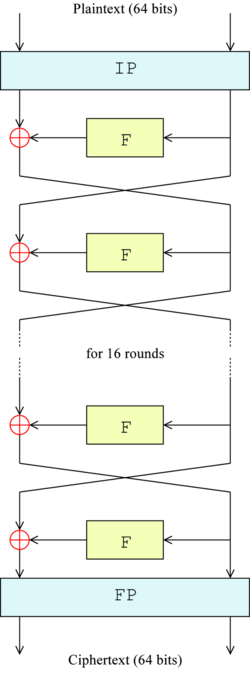
\includegraphics[width=5cm, angle=90]{informatika/siete_a_bezpecnost/obrazky/des-main-network.png}
    \caption{Schéma hlavní sítě algoritmu DES}
  \end{center}
\end{figure}

\begin{obecne}{Šifrování:}
\begin{pitemize}
	\item vstup projde iniciální permutací (IP:64b $\rightarrow$ 64b), na konci probíhá inverzní finální permutace (FP), následuje 16 identických kol šifrování:
	\item blok 64 bitů se rozdělí na dvě půlky po 32bitech, 
	\begin{pitemize}
		\item pravá půlka slouží jako vstup pro funkci F a také je v dalším kole použita jako levá část
		\item levá půlka se xoruje s výstupem funkce F a výsledek je použit v dalším kole jako pravá část
	\end{pitemize}
	\item celý cyklus se provede 16x a v závěru se ještě aplikuje finální permutace
\end{pitemize}
\end{obecne}

\begin{figure}[ht]
  \begin{center}
    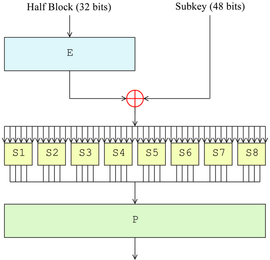
\includegraphics[width=6cm]{informatika/siete_a_bezpecnost/obrazky/des-f-function.png}
    \caption{Funkce \emph{F} v algoritmu DES}
  \end{center}
\end{figure}

\begin{obecne}{Funkce F:}
\begin{pitemize}
	\item ve funkci F probíhá míchání s klíčem. V každém kole vstupuje do funkce F 32bitů z \uv{pravé půlky} a 48bitový subklíč (odvozen z 56bitového klíče, detaily později).
	\item 32bitů z pravé půlky je nejprve expandováno na 48 bitů (fixní expanzní permutací, na obrázku označena E), potom xorováno se subklíčem. 
	\item Výsledek xorování se rozdělí na 8 bloků po 6bitech. Každý blok je pak vstupem jedné z osmi S funkcí. Každá S funkce převádí 6 bitů na 4 bity (nelineární transformací, \uv{zadrátované}).
	\item Výstupy S funkcí se opět spojí do jednoho bloku (8x4 = 32bitů) -- to je výsledek celé funkce F.
\end{pitemize}
\end{obecne}

\begin{obecne}{Dešifrování:} 
Díky prohazování poloviček v jednotlivých kolech lze dešifrování provádět stejnou funkcí (na stejném hardwaru), jako šifrování. Pouze je potřeba používat subklíče v opačném pořadí.
\end{obecne}

\begin{figure}[ht]
  \begin{center}
    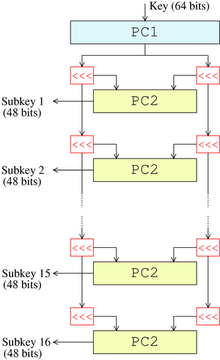
\includegraphics[width=6cm]{informatika/siete_a_bezpecnost/obrazky/des-key-schedule.png}
    \caption{Subklíče v algoritmu DES}
  \end{center}
\end{figure}

\begin{obecne}{Subklíče:}
\begin{pitemize}
	\item protože je klíč původně 64bitový, ale ve skutečnosti se používá pouze 56bitů (ostatní se zahazují, nebo slouží pro kontrolu parity), nejprve je vybráno těchto 56bitů funkcí PC1 (Permuted Choice 1) 
	\item Dále se vždy pro každé kolo 56 bitů rozdělí na dvě půlky po 28bitech. Každá z těchto půlek se bitově posune doleva (o jeden nebo dva bity, to je pevně určeno pro každé kolo). Takto posunuté půlky se vloží jako vstup funkce PC2, která vygeneruje 48bitový subklíč. Obě půlky také slouží jako vstup pro další kolo. 
	\item Algoritmus zaručuje, že každý bit z původního 56bitového klíče je použit asi ve 14-ti ze 16-ti subklíčů. 
	\item Pro dešifrování se klíče musí generovat v opačném pořadí (místo doleva se posouvá doprava).
\end{pitemize}
\end{obecne}



\end{document}
